\documentclass[10pt,twocolumn,letterpaper]{article}

\usepackage{cvpr}
\usepackage{times}
\usepackage{epsfig}
\usepackage{graphicx}
\usepackage{amsmath}
\usepackage{amssymb}
\usepackage{subfig}
\usepackage{booktabs} % for professional tables
\usepackage{adjustbox}

% Include other packages here, before hyperref.

% If you comment hyperref and then uncomment it, you should delete
% egpaper.aux before re-running latex.  (Or just hit 'q' on the first latex
% run, let it finish, and you should be clear).
\usepackage[breaklinks=true,bookmarks=false]{hyperref}

\cvprfinalcopy % *** Uncomment this line for the final submission


% Pages are numbered in submission mode, and unnumbered in camera-ready
%\ifcvprfinal\pagestyle{empty}\fi

\begin{document}

%%%%%%%%% TITLE
\title{Exploring User-friendly Retexturing of Semantic Image Subregions}

\author{Joshua Send \\
University of Cambridge \\
{\tt\small js2173@cam.ac.uk}
}

\maketitle


%%%%%%%%% ABSTRACT
\begin{abstract}

\end{abstract}

%%%%%%%%% BODY TEXT
\section{Introduction}

Modern data-driven machine learning has advanced computer vision and graphics greatly in the past few years. Examples abound, such as object detection~\cite{ren2015faster}, near-realistic photographic inpainting~\cite{li2017context}, 3D body position estimate~\cite{mehta2017vnect}, semantic segmentation~\cite{long2015fully}, and much more. One promise these advances hold is that non-expert users can utilize them for technical tasks which were previously impossible. 

As an example, a paper from Berkeley describes pix2pix~\cite{isola2017image}, in which convolutional neural networks (CNNs) are trained to convert between any two trained domains. One demonstration is that outline sketches of cats can be filled in and made realistic automatically by the system, using a large data set of sketches and cats seen before. Later advances allowed mapping between two unpaired, but grouped datasets (\eg one set of summer and winter pictures), demonstrating the ability to learn image features that are common within, and differentiate between two sets of images.

In the domain of image manipulation, a common task is retexturing or restyling particular regions. Manually, this involves selecting the desired region, and tediously pasting, transforming, and blending images together as required. Even with tools like Photoshop, much of this process still requires an expert user. This investigation explores what modern machine learning tools non-technical users might have at their disposal to manipulate image content. Specifically, the range of tasks between style transfer and texture transfer on image sub-regions is considered.

Two approaches to image manipulation are examined. The primary exploration utilizes a combination of semantic segmentation with networks generally used to transfer style between images. This approach is particularly appealing since users need minimal expertise to perform image manipulations: the only inputs are an image, an image subregion to manipulate, and a source style or texture image. The user can then modify how much weight is put towards the content of the base image (\ie its overall structure) versus the style image (\ie correlations between lower level features of the style image).

A second tangential exploration is performed using a conditional GAN called pix2pixHD~\cite{wang2017high}. This network is not entirely designed for the task at hand, as it converts semantic label mappings into realistic images (see Figure~\ref{fig:pix2pixHD} for an example). However, it is one of the few works available that enables a user to steer content generation, and as such is instructive as a platform for analysis. 

\begin{figure*}[t]
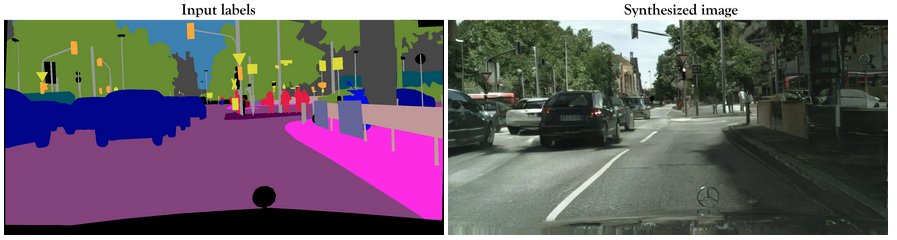
\includegraphics[width=\hsize]{images/pix2pixHD.png}
\caption{Pix2pixHD converts a semantic label map into a realistic synthesized image. Interestingly, content generation can be steered with a simple 3-dimensional feature vector per semantic class and instance. This example is from the Cityscapes dataset.}
\label{fig:pix2pixHD}
\end{figure*}

Thus, this paper contributes an application allowing restyling of subregions and an exploration of style transfer networks for style and higher level texture transfer on parts of an image. During the second investigation, a novel approach for fine tuning an existing, trained network with new examples is attempted, and the aforementioned GAN's ability to control content generation is examined in detail. A user study is used to rate both of these methods, along with a manual baseline, on their ability to achieve a desired retexturing, and realism of produced images.

\section{Related Work}

Visual content manipulation has a long history in the graphics and vision fields. A paper~\cite{simon1975digital} from 1975 considers image reconstruction in the context of satellite imagery, while a 1987 book is entirely dedicated to digital image processing~\cite{jensen1987introductory}, and automated perspective correction has been an active research area for nearly as long \cite{waltz1988implementation}.

This work focuses on automated style transfer, texture transfer, and visual content generation. The idea of separating style and content has recently been explored in depth, but the idea has been researched as far back as 2000. Style can be seen as the higher frequency features of an image, and representable as the correlation between different features -- for example, that edges are often at right angles in a particular image. Content can be seen as the higher level structure of an image, such as the outline of faces or regular patterns that emerge at larger scales.

An early approach to separating style and content using bilinear models fitted to training data utilized singular value decomposition and expectation maximization. It is surprisingly effective at creating fonts similar to existing styles\cite{tenenbaum1997separating}. However, their approach would struggle to extend to large images, and is not particularly adaptable to use different scales of style features or content features.

Much more recently, a highly cited approach using CNNs was published~\cite{gatys2016image}. In it, the authors use a standard network trained on ImageNet~\cite{ILSVRC15}, specifically VGG~\cite{simonyan2014very}, as means of extracting features from an image. The early convolutional feature activations represent local structure and can be combined with features from the later layers of the network to capture both local structure and large scale structure. These activations are formed into an outer product, creating the Gram matrix, representing the stylistic content of the image. The difference in Gram matrices is called the style loss. A content loss is defined separately from the difference in activations of a deep layer in the network. Style can then be transferred from one image to another by generating images that minimize a loss defined across content and style from two different images. This is the basis of the style and texture transfer network here. This work also explores tradeoffs in content and style when trying to redesign image subregions.

Texture synthesis and transfer is generally regarded as a separate problem, though it is treated jointly with style here. Many approaches have been proposed and used in the past. Some early work is highly mathematical, using wavelets ~\cite{portilla2000parametric} to to build a statistical model based on spatial locations, orientations, and scales. This is effective at regular texture synthesis, but the authors do not discuss transfer of texture. Other methods ``grow'' textures one pixel at a time from source image(s) by matching surrounding pixel statistics. This does not handle transfer either, and is prohibitively slow~\cite{efros1999texture}.

An impressive result is achieved in ~\cite{efros2001image}, sampling patches of the target texture based on similarity metrics, and splicing them together in a way that minimized some discontinuity penalty. Their results are difficult to tune between content and texture, and the user has to vary  parameters to achieve minimal edge-boundary discontinuity. Even more impressive are the results from~\cite{diamanti2015synthesis}, in which the authors a set of input textures annotated with surface normals to handle texture transfer to even non-planar surfaces. However, this is hardly conforming to our goal of providing user-friendly tools.

The second direction this investigation takes is exploring a network that allows users to steer realistic content generated by a generative adversarial network (GAN). GANs are a method for training both a generator and discriminator in tandem, resulting in networks that effectively learn the manifold of realistic data, mapping random noise as inputs onto it. Conditional adversarial networks provide an extra input to both the generator and discriminator during training. At test time, this allows steering content generation via the additional input. The GAN used here, pix2pixHD allows adding a 3-dimensional feature vector per semantic class that represents a certain style to be generated. This feature space is explored in depth.

In Section TODO I will describe an attempt to fine tune the GAN on a slightly extended training set. This is inspired by recent work on learning rate schedules. In particular~\cite{loshchilov2016sgdr}, which describes training of neural networks using cosine-learning rate decay, utilizing a high learning rate to leave a local minimum and driving down quickly to converge to an alternative one. 

\section{Implementation}
\label{sec:implementation}

The core part of this paper involves two components: a segmentation network and style transfer. A pretrained segmentation network is used, PSPNet~\cite{zhao2017pyramid}, which won the 2016 ImageNet scene parsing challenge. The second part is a CNN based on the Keras sample implementation of style transfer. This in turn is based on~\cite{gatys2016image}. The evaluation consists of experimenting with various settings of this network. The restyled image is then merged with the original by cropping out the segmented region, blending the edges of the restyled portion for realism.

The pix2pixHD GAN was obtained from~\url{https://github.com/NVIDIA/pix2pixHD}, though it was not available pre-trained, thus the network had to be trained from scratch on the Cityscapes~\cite{cordts2016cityscapes} dataset. The feature space encoding is learned through an encode-decoder architecture that is trained in tandem with the generator and discriminator networks. This network is of most interest to us: it takes as input an image and its semantic labeling, and outputs an average `feature' for each semantic region, representing a style. This can be fed into the generator network along with a semantic labeling to generate images of the corresponding style.

The architecture or losses used in pix2pixHD will not be described further, for more information please refer to~\cite{isola2017image}. Training this GAN is extremely time consuming and thus only trained for 100 instead of the author's 200 epochs, resulting in slightly less realistic images.

Armed with a trained generator and feature encoder network, I explore various aspects of the feature space. All training images are run through the encoder, resulting in approximately one feature per present semantic class per image (30 classes total in the Cityscapes dataset). I mainly analyze the `road' semantic class. There are 5000 road instances in the training set. These are clustered using k-means to find ``average'' styles of roads TODO REF. They are also clustered using furthest-first clustering to examine the most disparate road styles possible, see Section TODO.


\section{Results}

Most of this section will focus on applying a \textit{yellow brick road} texture to roads from the Cityscapes dataset. Other examples will be scattered in to demonstrate a wider range of applicability. 

A user study was performed testing results obtained from manual, style network, and GAN, asking users to rate a randomly ordered selection of images on firstly realism (referred to a Q1), and secondly how well the image depicts a yellow brick road (Q2). These results are given in the corresponding sections. 37 responses were collected from students at my college and within the computer science masters program. Ratings were given from 1 (not realistic/not like a yellow brick road) to 5 (very realistic/like a yellow brick road).

\subsection{Manual Baseline}
\label{sec:manual}
I present three examples of manually converted images, changing brick roads into various types of yellow brick roads.

In Figure~\ref{fig:manual}, the first two examples were rather time consuming, requiring outlining, perspective shifting, expanding the texture, and cloning. The last was rather simple, only requiring outlining and color space shifting. We will see below though that it is not deemed to look much like a yellow brick road.

\begin{figure}
	\subfloat[Source]{
		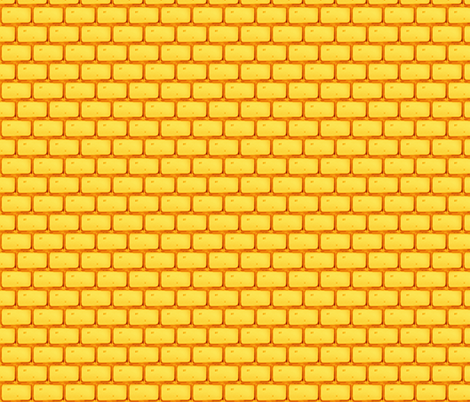
\includegraphics[width=0.3\hsize]{images/manual/yellow_bricks_reddish.png}
		\label{fig:manual:a}
	}
	\subfloat[Result]{%
		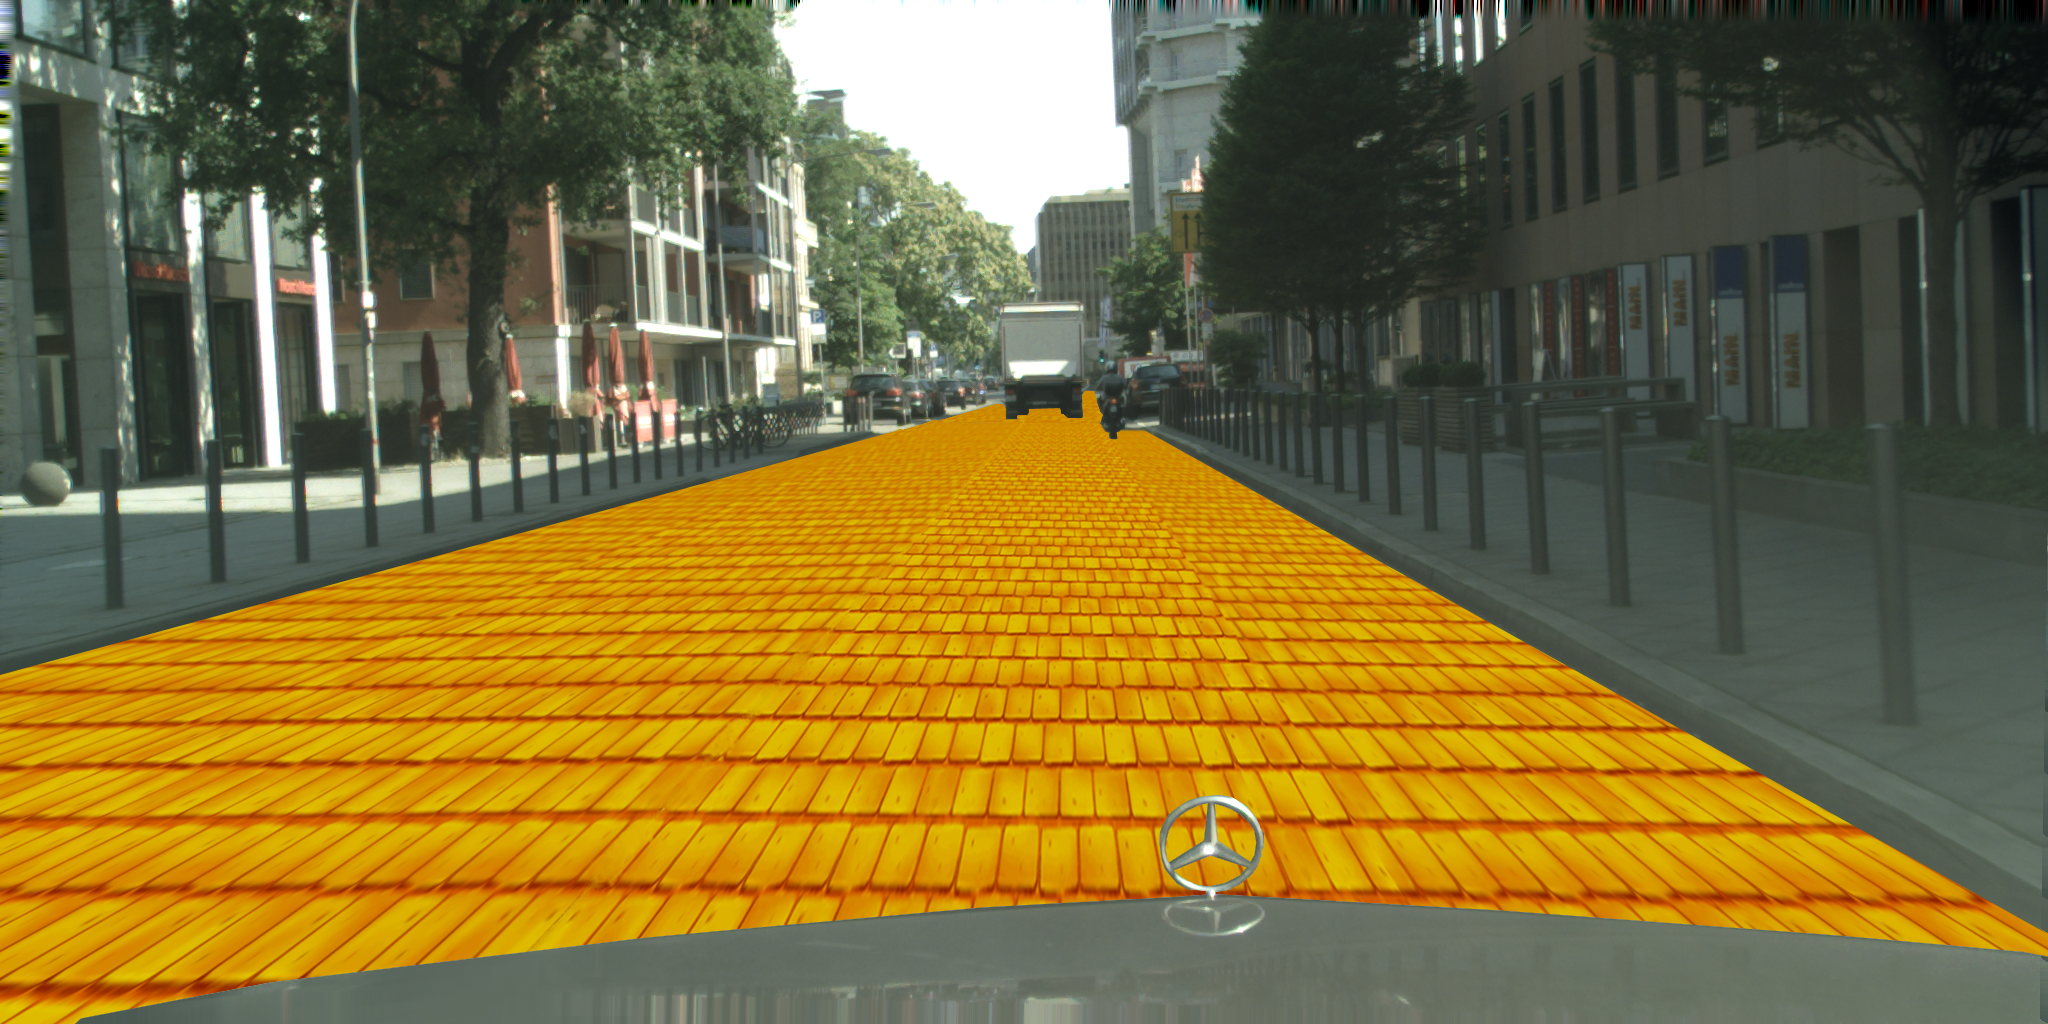
\includegraphics[width=0.7\hsize]{images/manual/reddish.png}
		\label{fig:manual:b}
	}
	
	\subfloat[Source]{
		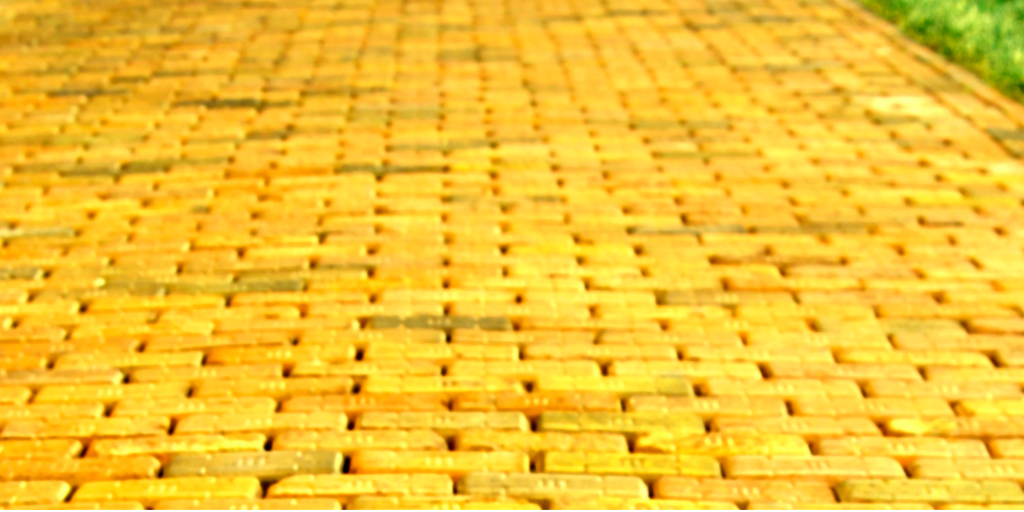
\includegraphics[width=0.3\hsize]{images/manual/yellow_bricks.png}
		\label{fig:manual:c}
	}
	\subfloat[Result. Note the lack of realistic shadows.] {
		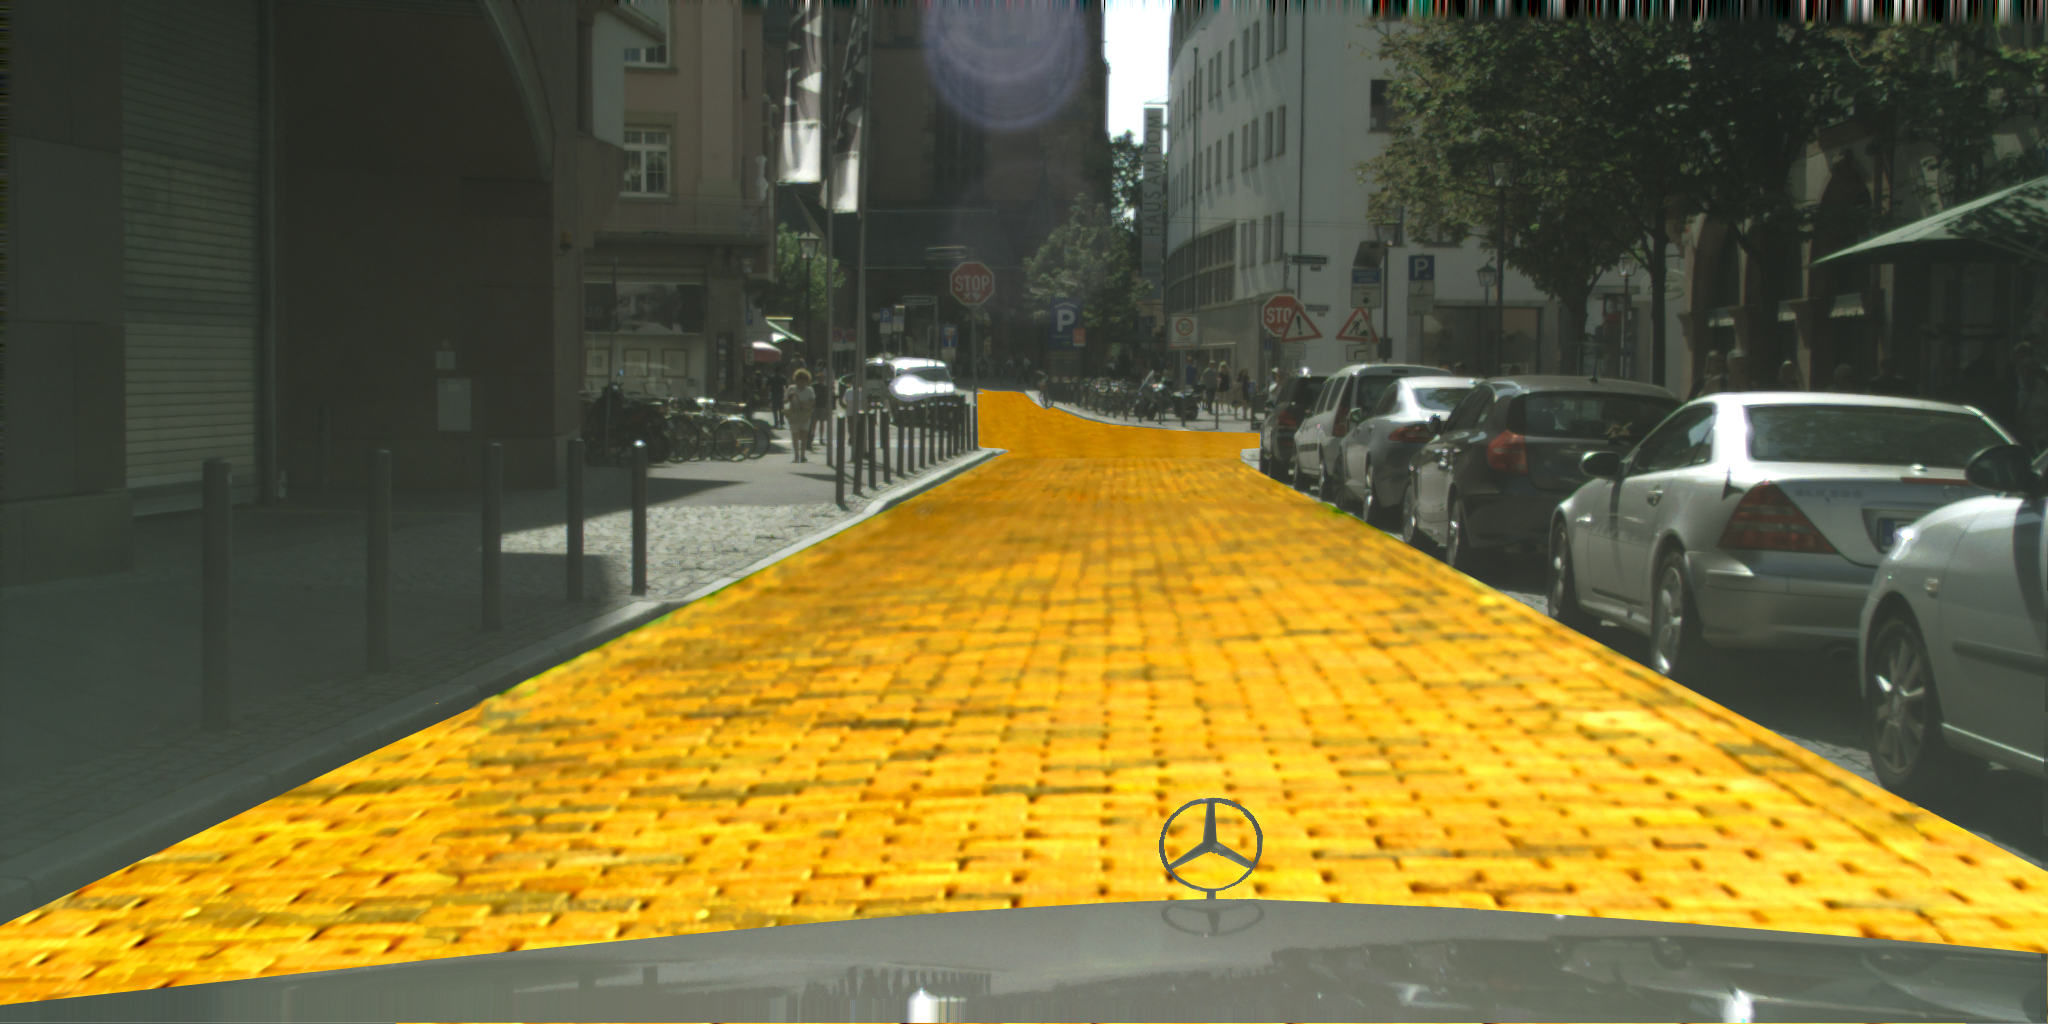
\includegraphics[width=0.7\hsize]{images/manual/result_sat.png}
		\label{fig:manual:d}
	}
	
	\subfloat[A result obtained by selecting the road and shifting its color space.] {
		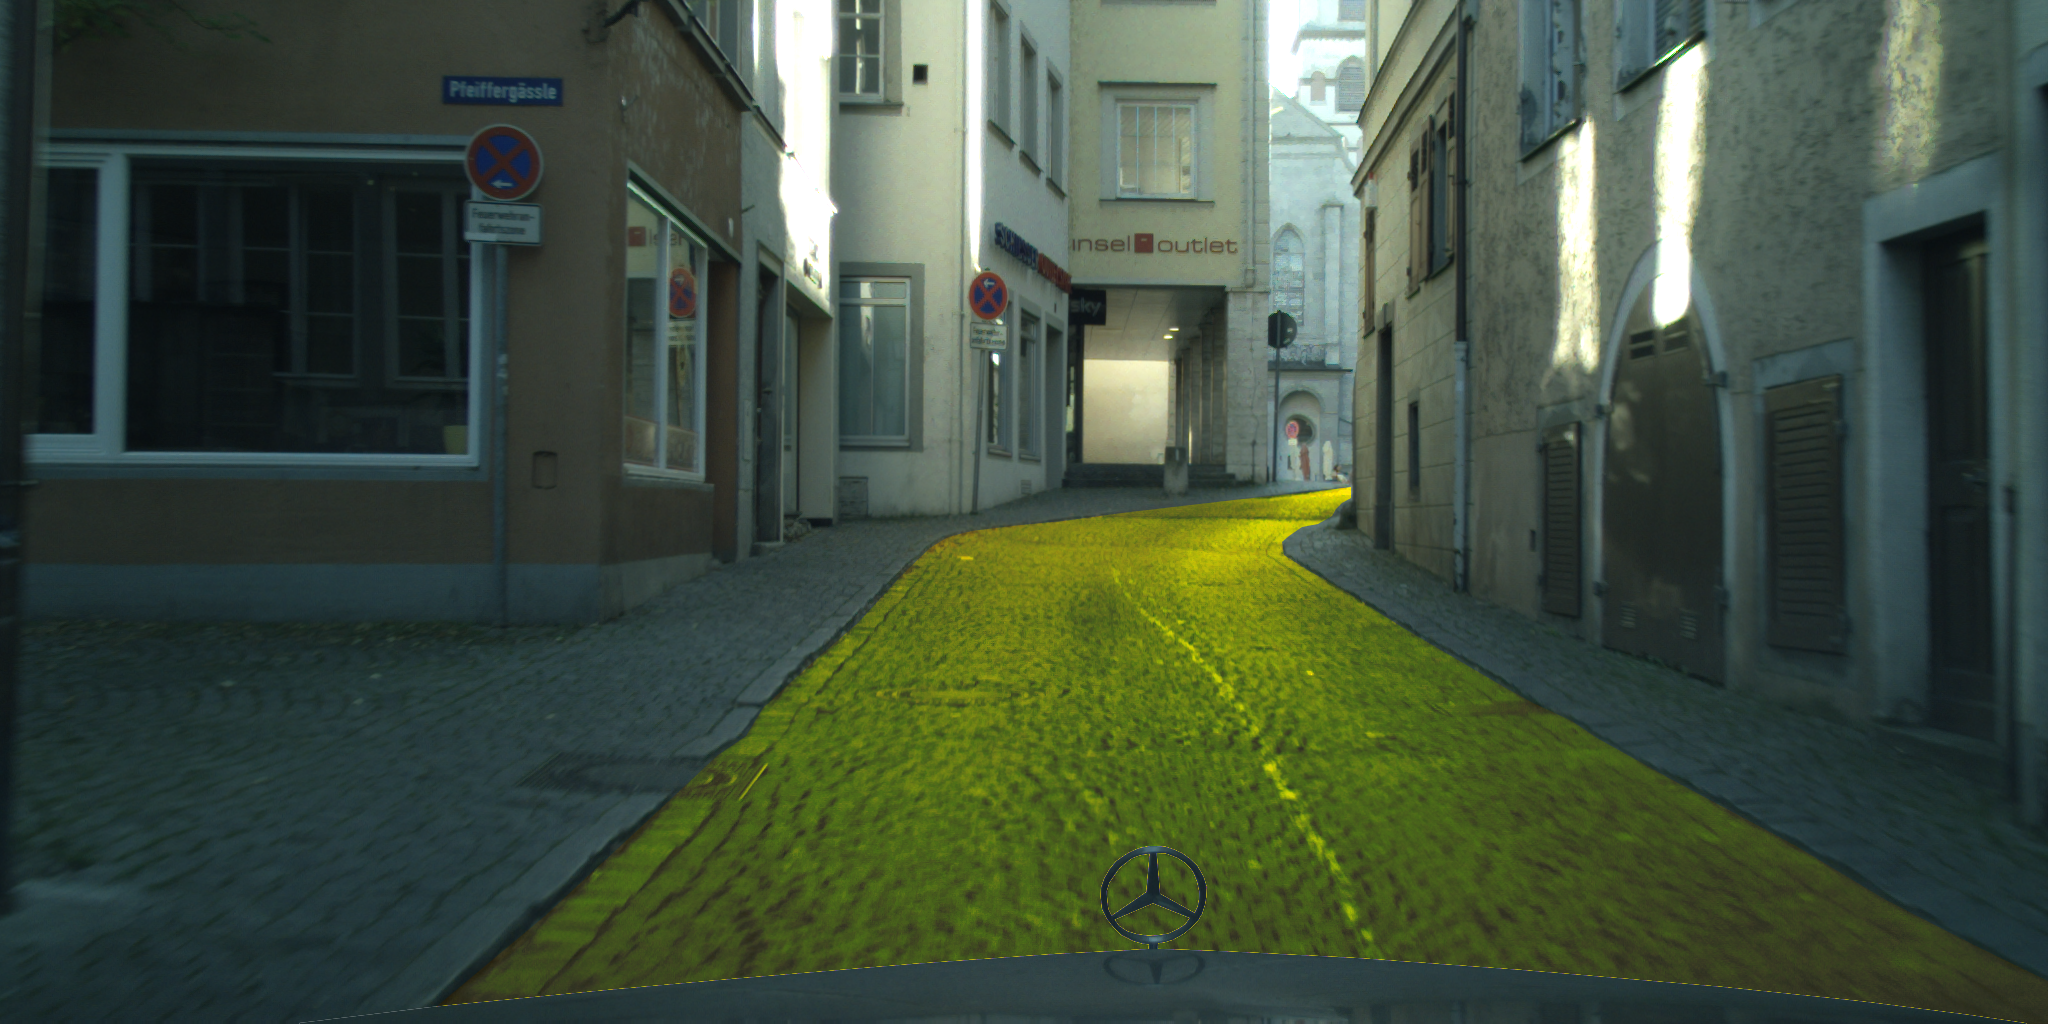
\includegraphics[width=\hsize]{images/manual/colorspace.png}
		\label{fig:manual:e}
	}
	\caption{}
	\label{fig:manual}
\end{figure}


\begin{table}[htb]
\caption{Mean $\pm$ 1 standard deviation survey responses to realism (Q1) and likeness of a `yellow brick road' (Q2) for manual editing, on a scale of 1 to 5.}
\vskip 0.15in
\begin{center}
\begin{small}
\begin{sc}
\begin{tabular}{lccr}
\toprule
Figure				 		& Q1	& Q2 \\
\midrule
Figure~\ref{fig:manual:b} 	& $1.86 \pm 0.89$	& $3.92 \pm 1.04$  \\
Figure~\ref{fig:manual:d}	& $2.40 \pm 0.86$	& $4.18 \pm 0.84$  \\
Figure~\ref{fig:manual:e}	& $3.40 \pm 0.98$	& $3.62 \pm 1.01$  \\
\bottomrule
\end{tabular}
\end{sc}
\end{small}
\end{center}
\vskip -0.1in
\label{tab:model_accuracies}
\end{table}

The survey shows that the top image scores relatively well on looking like a yellow brick road, but is hardly realistic. The last image is more realistic, but less like a yellow brick road, and the middle entry looks very much like a yellow brick road and has middling realism.



\subsection{Segmentation + Neural Style Transfer}

\subsubsection{Standard Style Transfer}
I first confirm that the normal use case for neural style transfer works as hoped. As a style I use Van Gogh's \textit{Starry Night}, transferred onto the road section of a Cityscapes image. Figure~\ref{fig:starry} shows this works reasonably well, extracting color and what could be seen as stroke style and applying to the desired region. Because the style is relatively sparse, edge blending is not required to make a visually appealing result.

\begin{figure}[htb]
	\subfloat[Source]{
		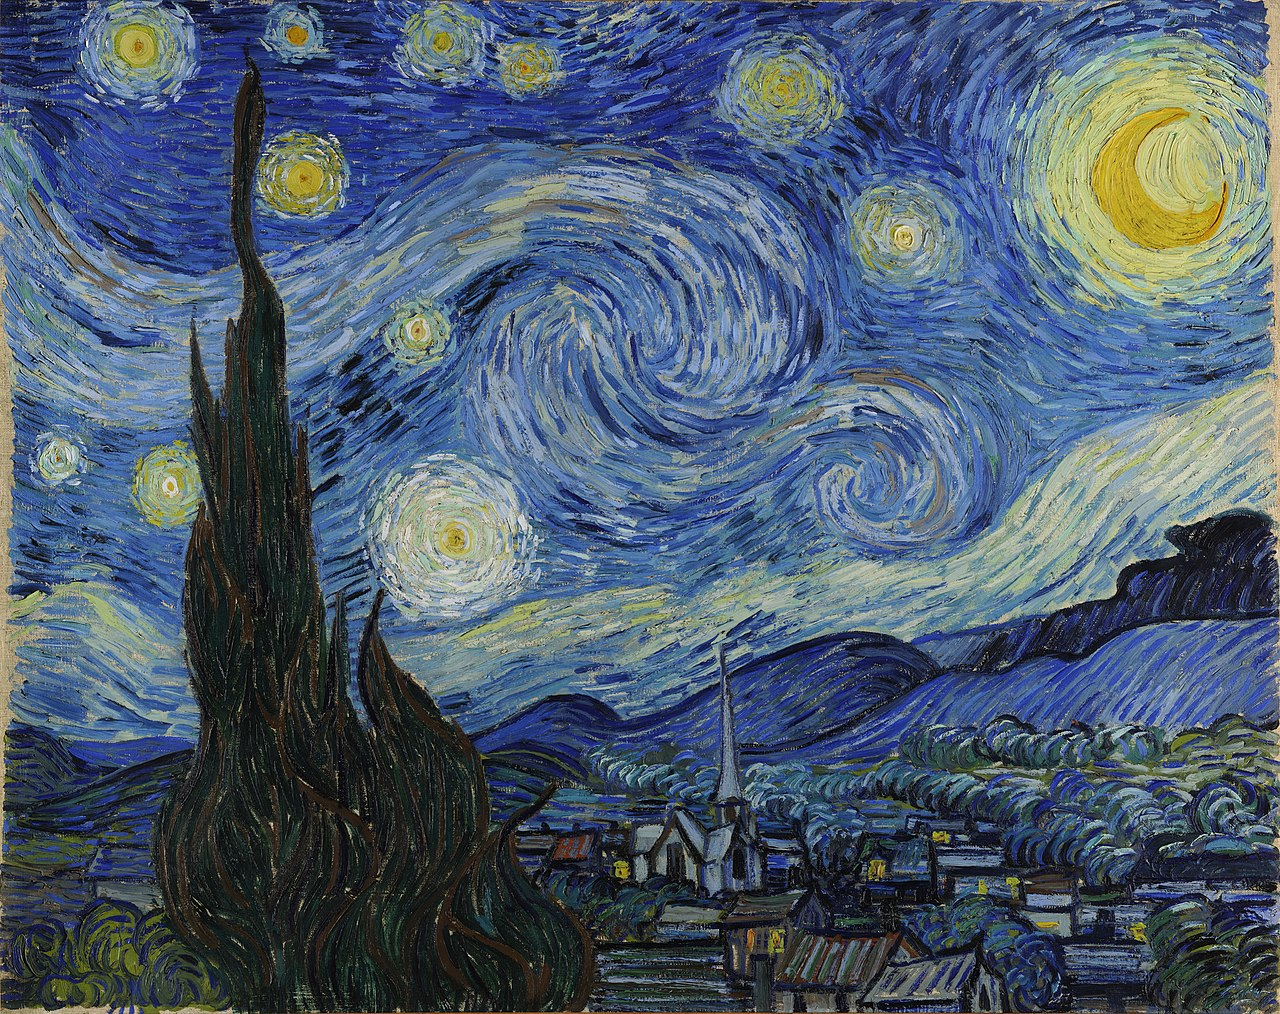
\includegraphics[width=0.25\hsize]{images/results/starry_night.jpg}
		\label{fig:starry:a}
	}
	\subfloat[Result]{%
		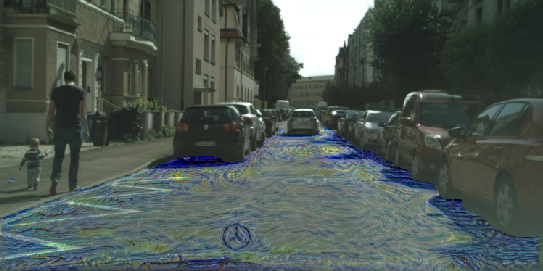
\includegraphics[width=0.75\hsize]{images/results/starry_night_retexture.png}
		\label{fig:starry:b}
	}
	\caption{Transferring Starry Night styles onto a road.}
	\label{fig:starry}
\end{figure}

From this we can reasonably conclude that transferring styles defined by small, high frequency components such as local color and strokes can be very effectively done for image subregions (at least on planar surfaces).

\subsubsection{Texture Transfer -- Loss Design}
In this case we define texture as a style with larger scale structure, such as one might find on roads or other surfaces. The challenge here is to preserve some of the higher level details beyond just color and small edges.

Consider the algorithm that neural style transfer is based on: it computes correlations between features at selected levels of a neural network. CNNs have increasing large receptive fields in deeper layers of the network, so we hope that we can reproduce texture in a similar manner as style by using mostly high level activations from the VGG network, corresponding to more structured, large scale image features.


\begin{figure}
	\subfloat[Desired Texture]{
		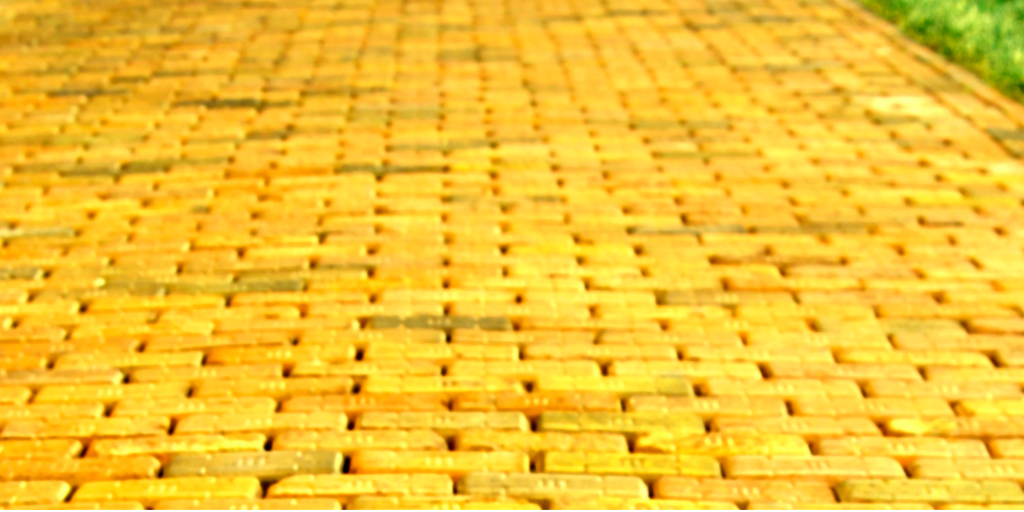
\includegraphics[width=0.5\hsize]{images/manual/yellow_bricks.png}
		\label{fig:texture:source}
	}
	\subfloat[Target image]{
		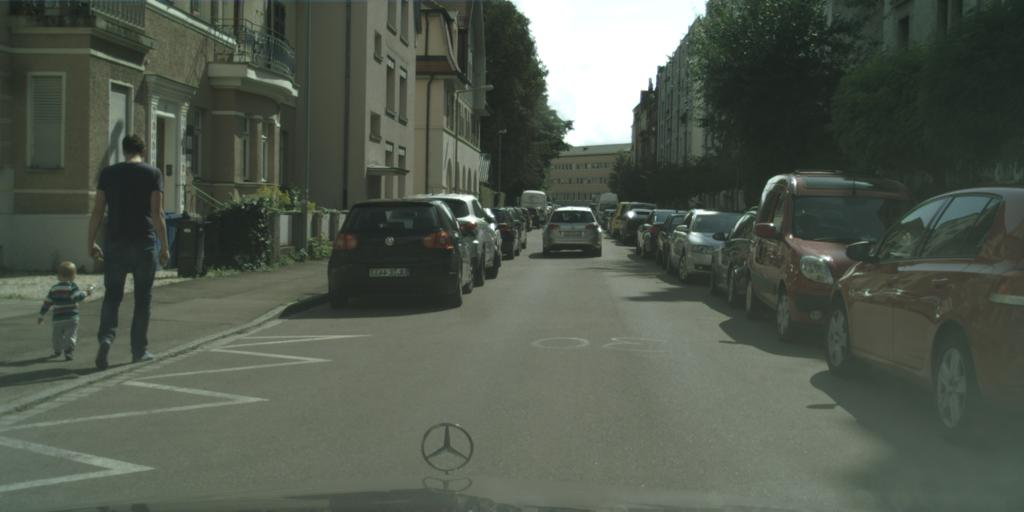
\includegraphics[width=0.5\hsize]{images/results/epoch100_real_image.jpg}
		\label{fig:texture:target}
	}
	\caption{Goal: Transfer the texture on the left onto the road in the right image.}
\end{figure}

The goal is to transfer the texture in~\ref{fig:texture:source} to~\ref{fig:texture:target}. To determine which layers should be used to form the style loss, I run the style transfer network on empty images using individual layers in the network. Some of the results are shown in Figure~\ref{fig:activations}. From here I choose parts of the style that I consider relevant: some of the early ones to encourage the correct color (layers 1 and 2), and high level ones to maintain structure (14, 15, 17, 18).

\begin{figure}
	\subfloat[VGG Layer 1]{
		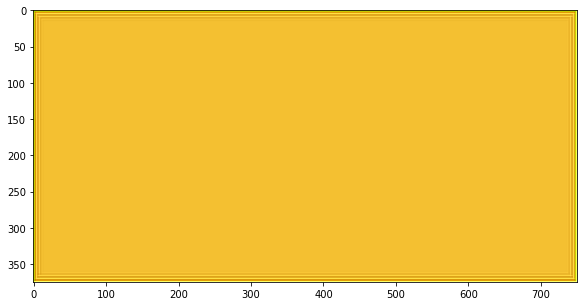
\includegraphics[width=0.5\hsize]{images/results/yellow_bricks_activations/1.png}
		\label{fig:activations:1}
	}
	\subfloat[VGG Layer 2]{
		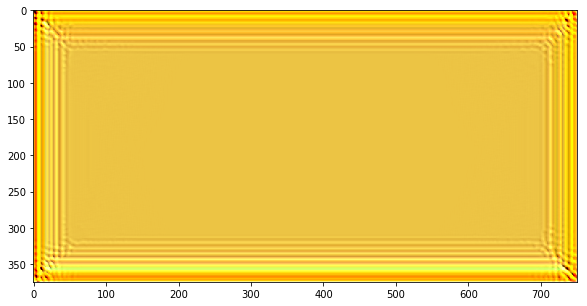
\includegraphics[width=0.5\hsize]{images/results/yellow_bricks_activations/2.png}
		\label{fig:activations:2}
	}
	
	\subfloat[VGG Layer 4]{
		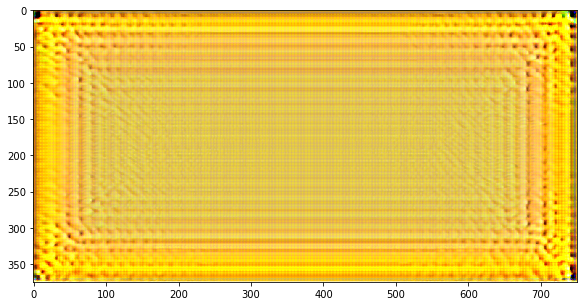
\includegraphics[width=0.5\hsize]{images/results/yellow_bricks_activations/4.png}
		\label{fig:activations:4}
	}
	\subfloat[VGG Layer 5]{
		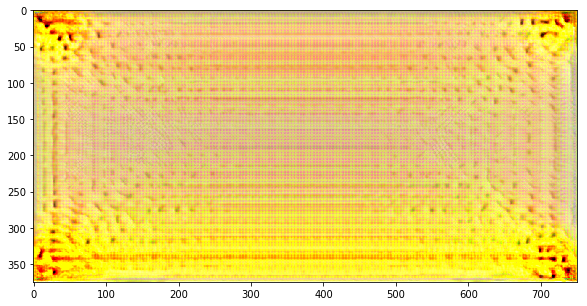
\includegraphics[width=0.5\hsize]{images/results/yellow_bricks_activations/5.png}
		\label{fig:activations:5}
	}
	
	\subfloat[VGG Layer 8]{
		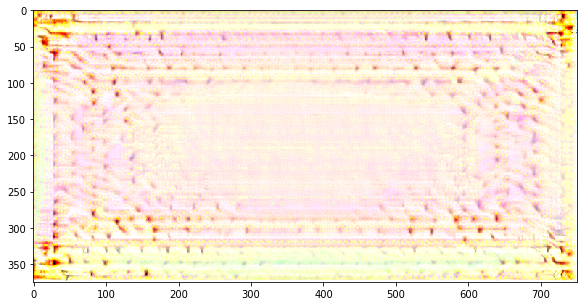
\includegraphics[width=0.5\hsize]{images/results/yellow_bricks_activations/8.png}
		\label{fig:activations:8}
	}
	\subfloat[VGG Layer 12]{
		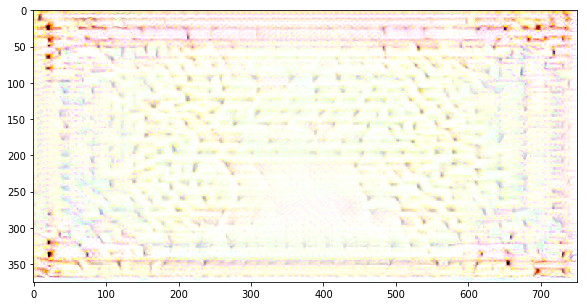
\includegraphics[width=0.5\hsize]{images/results/yellow_bricks_activations/12.png}
		\label{fig:activations:12}
	}
	
	\subfloat[VGG Layer 13]{
		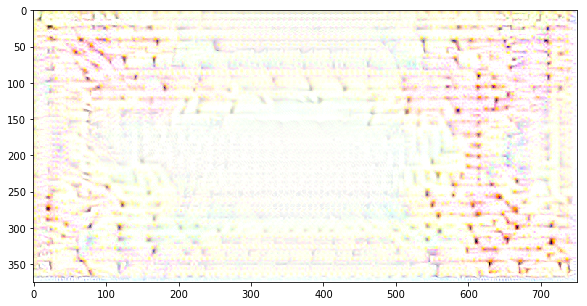
\includegraphics[width=0.5\hsize]{images/results/yellow_bricks_activations/13.png}
		\label{fig:activations:13}
	}
	\subfloat[VGG Layer 14]{
		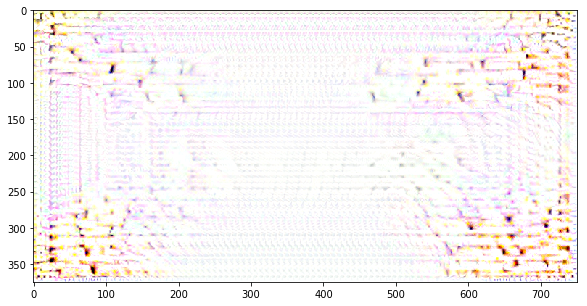
\includegraphics[width=0.5\hsize]{images/results/yellow_bricks_activations/14.png}
		\label{fig:activations:14}
	}
	
	\subfloat[VGG Layer 15]{
		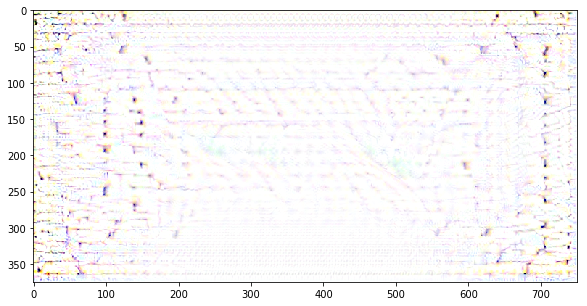
\includegraphics[width=0.5\hsize]{images/results/yellow_bricks_activations/15.png}
		\label{fig:activations:15}
	}
	\subfloat[VGG Layer 18]{
		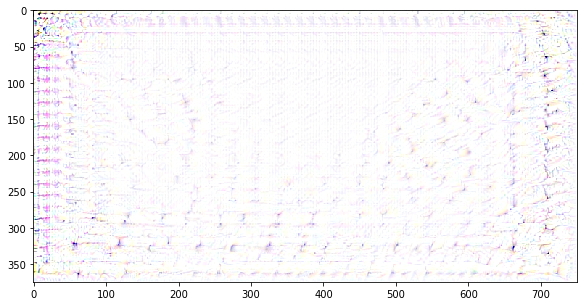
\includegraphics[width=0.5\hsize]{images/results/yellow_bricks_activations/18.png}
		\label{fig:activations:18}
	}
	
	\caption{Style transfer from selected layers of VGG onto an empty image.}
	\label{fig:activations}
\end{figure}

The result of applying semantic segmentation to the road, cropping a bounding box around it, applying texture transfer, re-inserting the restyled road, and interpolating the edges to blend the results together can be seen in Figure~\ref{fig:retextured}. 

\begin{figure}[htb]
	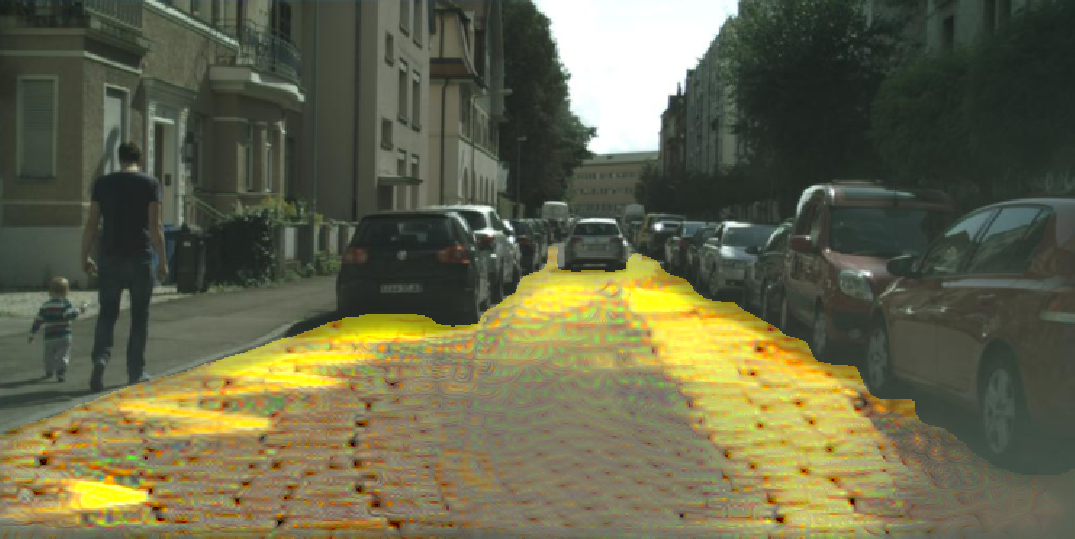
\includegraphics[width=\hsize]{images/results/decent_texture_transfer_sw_100-tv_0-cw_0-01.png}
	\caption{Result of using neural style transfer for texture transfer, after smoothing edges.}
	\label{fig:retextured}
\end{figure}

We can see that the transfer is not entirely successful: yellow bricks are identifiable, though not clearly defined, and shadows are preserved from the original image. Some regions are too bright, while the center of the road lacks texture. This is explained by Figure~\ref{fig:activations:13}, in which the VGG network does not respond as much to structure in the center of an image as toward the edges.

Ultimately, I found that the layer selection did not have a huge effect as long as early and deep layers are well represented in the loss function, and that the image is cropped and blended back together. 

\subsubsection{Texture Transfer -- Loss Weighting}

The second important aspect of this process is the tradeoff between content loss (\eg how similar the produced image is to the original image), style loss (defined above), and total variation loss (a quantification of overall smoothness). To achieve the above result, the variational loss weight is set to 0 -- we want to discourage overly smooth results. This is very different from the weighting used for style transfer.


\begin{table}[htb]
\caption{Mean survey responses to realism (Q1) and likeness of a `yellow brick road' (Q2) Low versus High variational loss weight.}
\vskip 0.15in
\begin{center}
\begin{small}
\begin{sc}
\begin{tabular}{lccr}
\toprule
Variational Loss Weight		& Q1				& Q2 \\
\midrule
Low 	& $1.85$	& \textbf{2.54}  \\
High 	& $1.81$	& 1.85  \\
\bottomrule
\end{tabular}
\end{sc}
\end{small}
\end{center}
\vskip -0.1in
\label{tab:tvweight}
\end{table}

A user study was conducted which of these weights are more important for realism and effectiveness at recreating a yellow brick road. Three images were presented with different yellow brick textures, each with 3 variations on the weightings. Table~\ref{tab:tvweight} shows that the total variational loss is not particularly important to realism, but has a large impact on how well the target texture is represented. This is further evidence setting the variational loss weight close to or equal to 0 results in more realistic images.

\begin{table}[htb]
\caption{Mean survey responses to realism (Q1) and likeness of a `yellow brick road' (Q2) Low versus High style loss weight.}
\vskip 0.15in
\begin{center}
\begin{small}
\begin{sc}
\begin{tabular}{lccr}
\toprule
Style Loss weight				& Q1				& Q2 \\
\midrule
Low 	& $1.60$	& $2.23$  \\
High 	& $2.34$	& $2.84$  \\
\bottomrule
\end{tabular}
\end{sc}
\end{small}
\end{center}
\vskip -0.1in
\label{tab:stweight}
\end{table}

The limited user study quantified in Table~\ref{tab:stweight} suggests that style weighting is a major factor in determining realism and likeness to the target texture. A style weight of 100.0 is used here. Content weight was determined beforehand to have a smaller effect on the final image and is set to 0.01, and not examined in the user study.

\subsubsection{Conclusion}


\begin{figure}[htb]
	
	\subfloat[Texture]{
		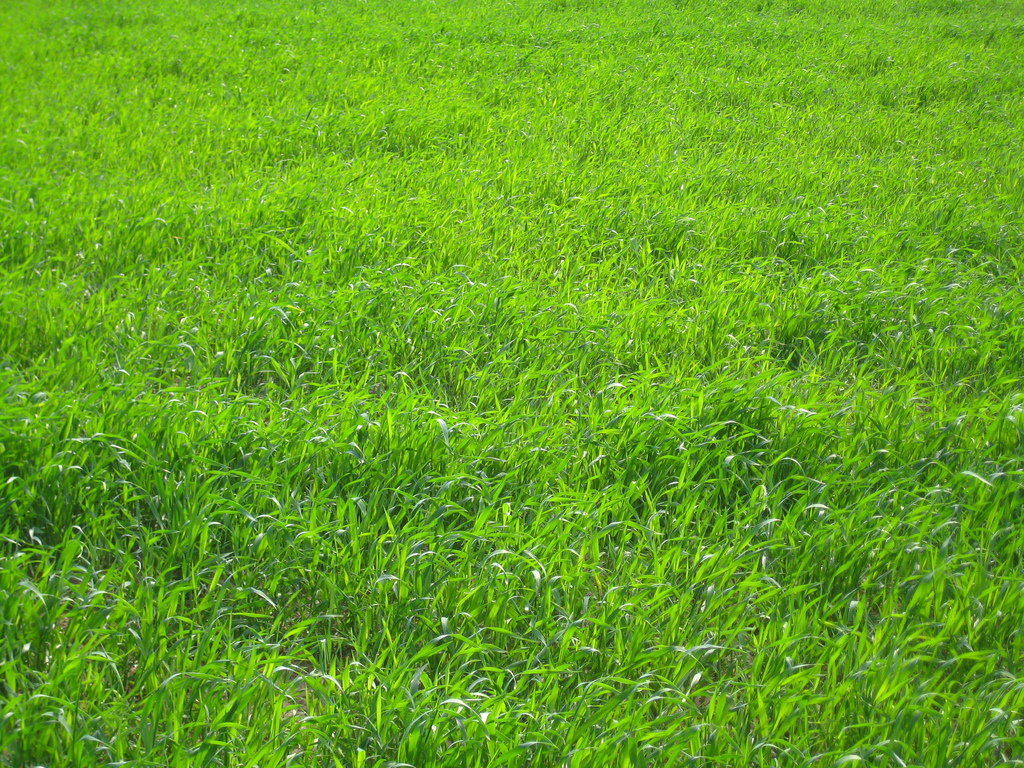
\includegraphics[width=0.25\hsize]{images/results/grass.jpg}
		\label{fig:grass_texture}
	}
	\subfloat[result]{
		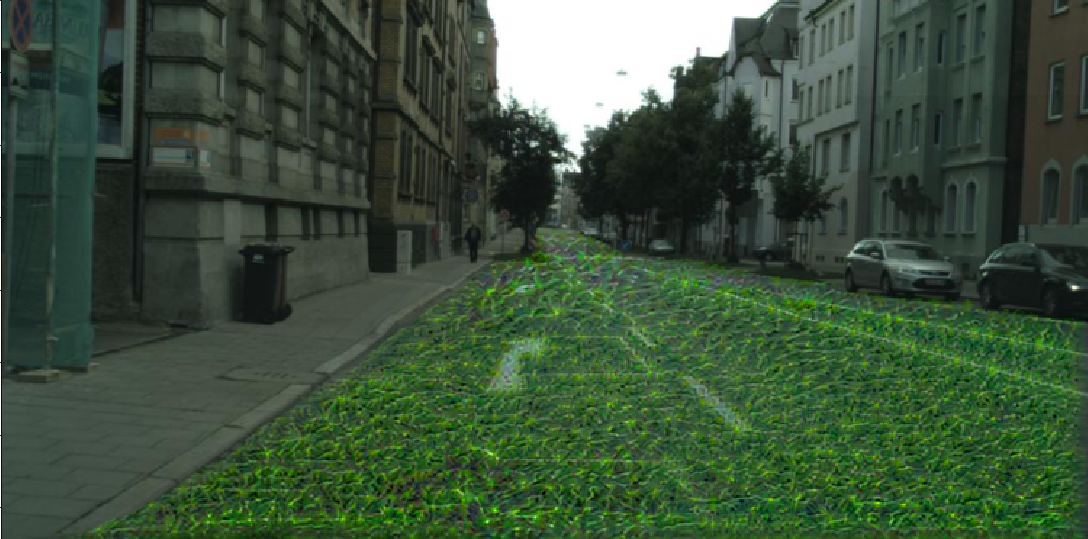
\includegraphics[width=0.75\hsize]{images/results/grass_road.png}
		\label{fig:grassy}
	}
		
	\subfloat[Texture]{
		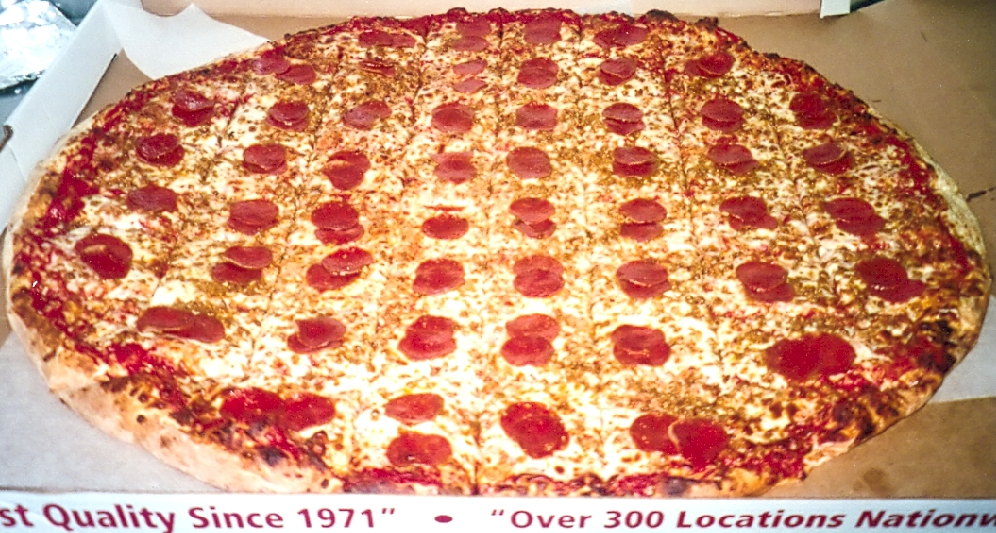
\includegraphics[width=0.25\hsize]{images/results/pizza.png}
		\label{fig:pizza_texture}
	}
	\subfloat[Result]{
		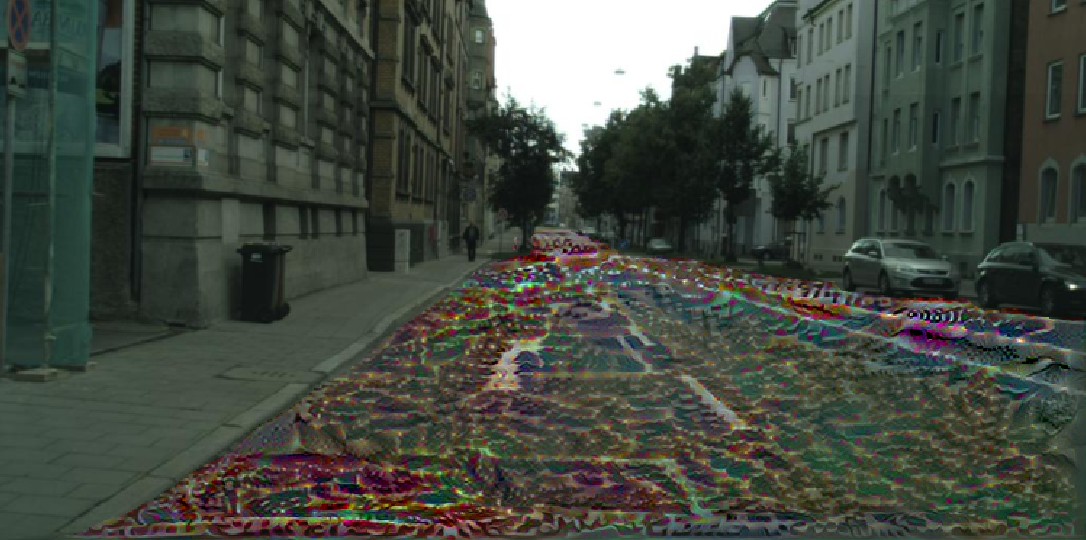
\includegraphics[width=0.75\hsize]{images/results/pizza_road.png}
		\label{fig:pizza}
	}
	\caption{Other textures applied to a different road scene. The total variation loss weight was increased to 0.01 to generate these results.}
	\label{fig:otherstyles}
\end{figure}

This section has explored the use of a neural style transfer network as both a style and texture transfer mechanism for image subregions. Overall, I conclude that neural style transfer is capable of handling coarse texture transfer, but fails to offer definition or regularity, even after tuning the style loss components and loss weightings. The main benefit of this method is its ease of use, requiring only requiring two images to get started; users would be offered an interface for tuning the VGG layers that feed into the style loss and manipulating the loss weights.





\subsection{Semantic Image Manipulation using GANs}

The pix2pixHD GAN was introduced in Section~\ref{sec:implementation}. Once the GAN is trained, we are interested into the generator and the encoder, which takes an image, a semantic label map, and returns a 3-dimensional vector\footnote{The dimensionality can be set during training, though 3 is the default} per semantic region representing style.

This is particularly interesting since users can choose a style feature vector for a region and the target output will be generated in a photo-realistic setting. The downside to this approach is that the networks must have seen the target style to be able to generate it. 


\begin{figure}[htb]
	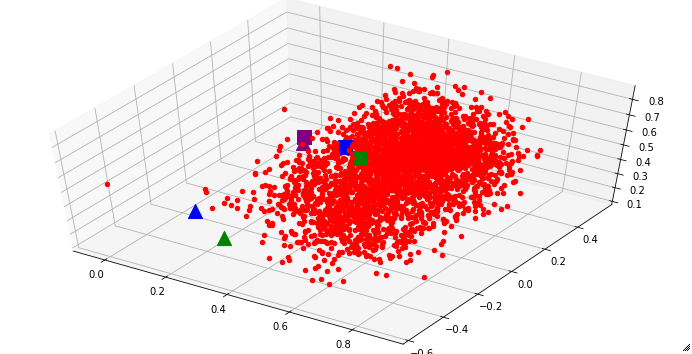
\includegraphics[width=\hsize]{images/feature_space.png}
	\caption{The feature space encoding of all roads in the training set. The large colorful points represent yellow brick roads encoded through the same encode-decoder network. Triangles represent yellow brick roads in color, while squares of the same color are desaturated, grayscale ``yellow'' brick roads to demonstrate the encoder also learns to recognize color.}
	\label{fig:feature_space}
\end{figure}

Knowing that the network was not trained on yellow bricks roads, I encoded the three manually edited yellow brick roads introduced in Section~\ref{sec:manual}. In Figure~\ref{fig:feature_space}, these are shown as the large colorful squares. Two are far from the point cloud, while the third (purple) has been mapped to a point closer toward the center.

\begin{figure}
	\centering
	\subfloat[Generated image using feature vector extracted from road in upper right image. No yellow is present, though some sort of cobble/slate road is the nearest style the networks can generate.]{
		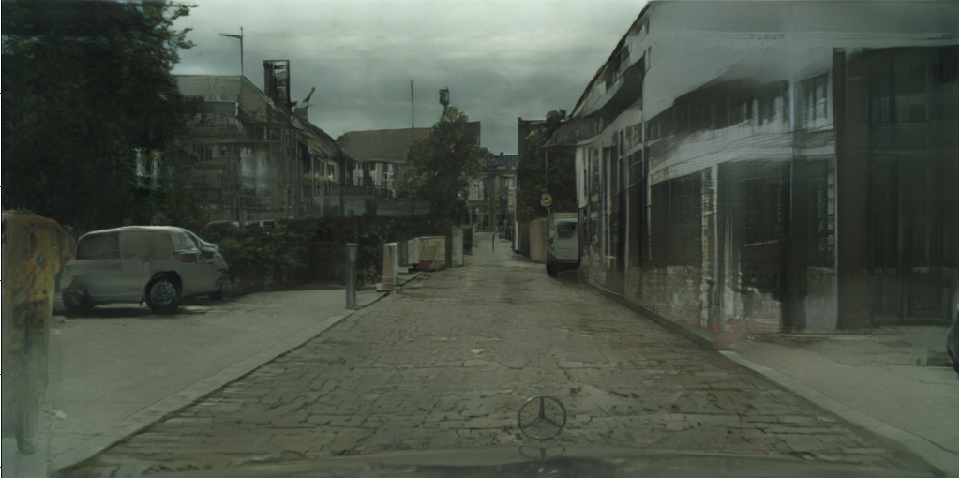
\includegraphics[width=0.9\hsize]{images/reddish_colorized_generated.png}
		\label{fig:gan:gen_a}
	}
	\subfloat{
		\hspace{-4cm}
		\raisebox{11ex}[0pt][0pt]{
			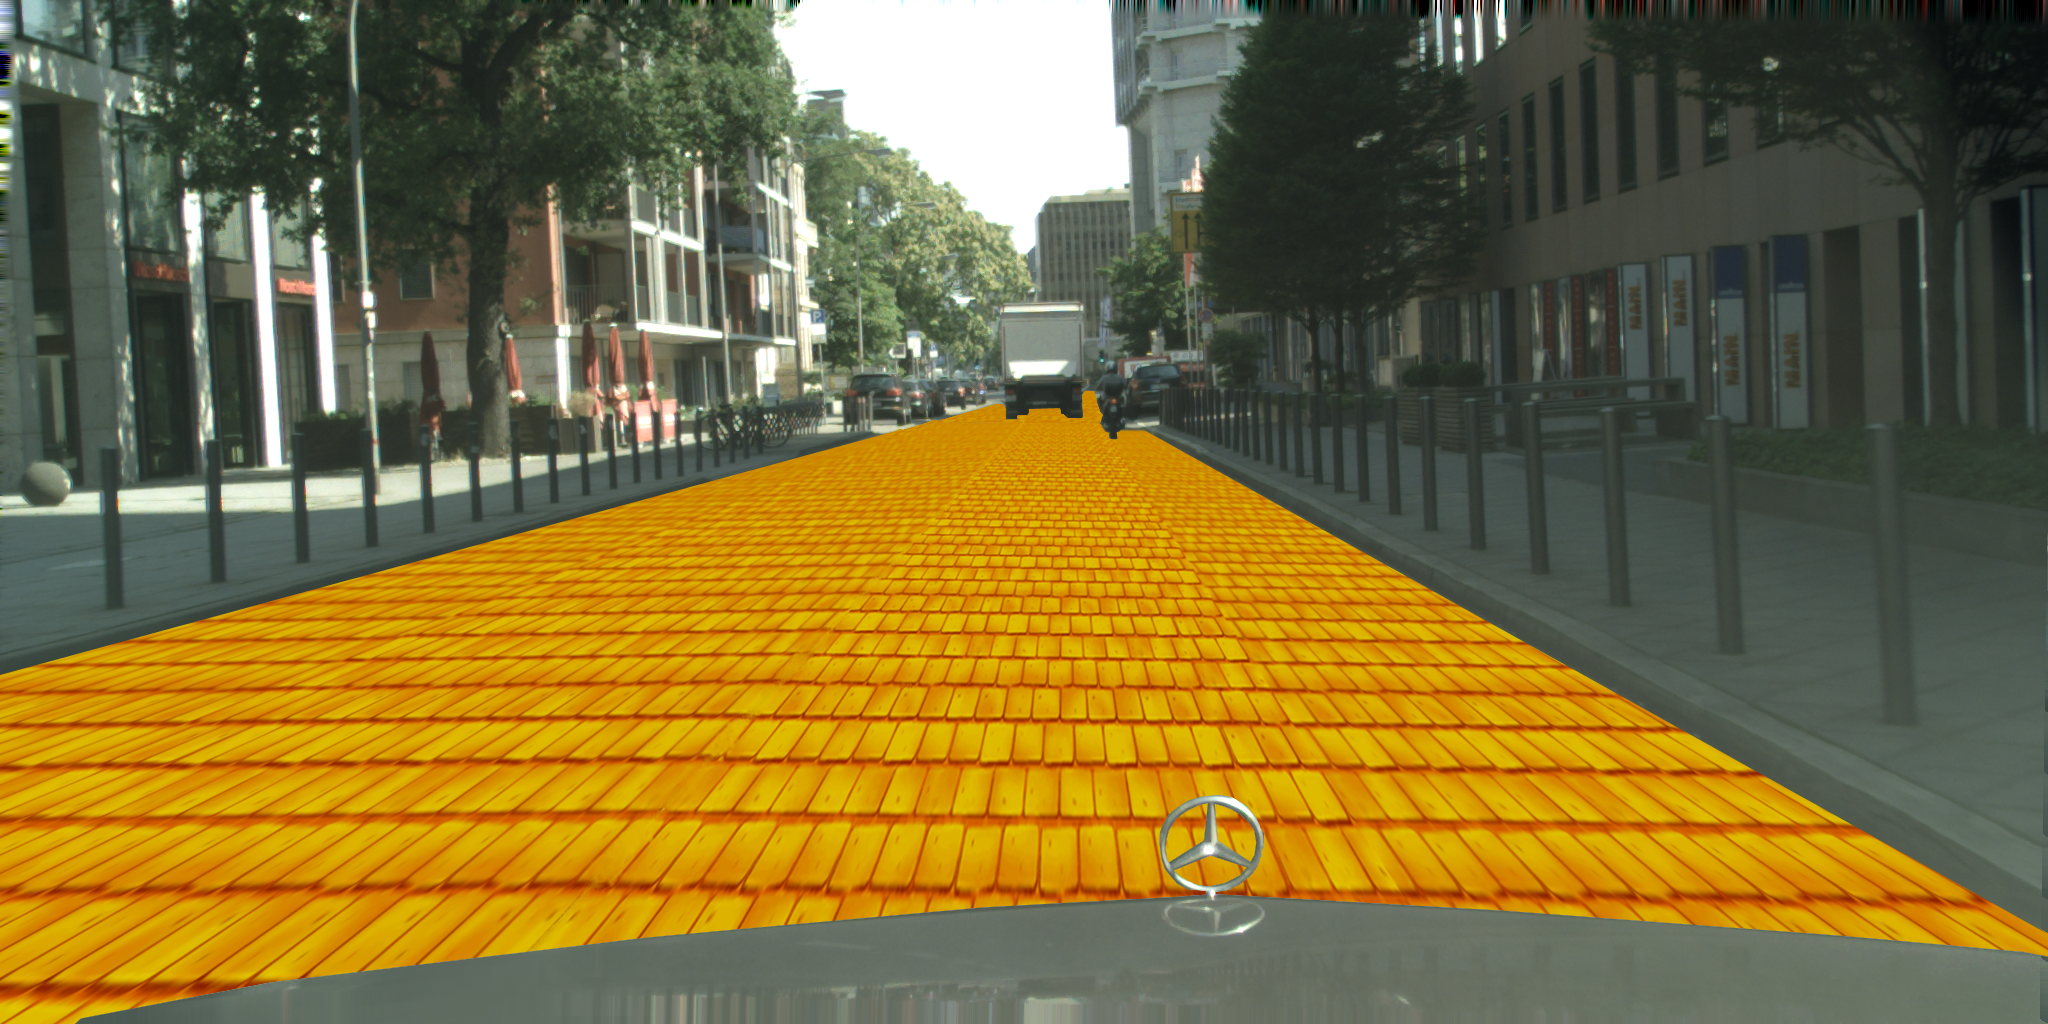
\includegraphics[width=0.5\hsize]{images/manual/reddish.png}
		}
	} 
	
	\subfloat[Corresponds to purple markers in~\ref{fig:feature_space}. This feature vector is relatively central and fails to capture even similarity with cobblestones.]{
		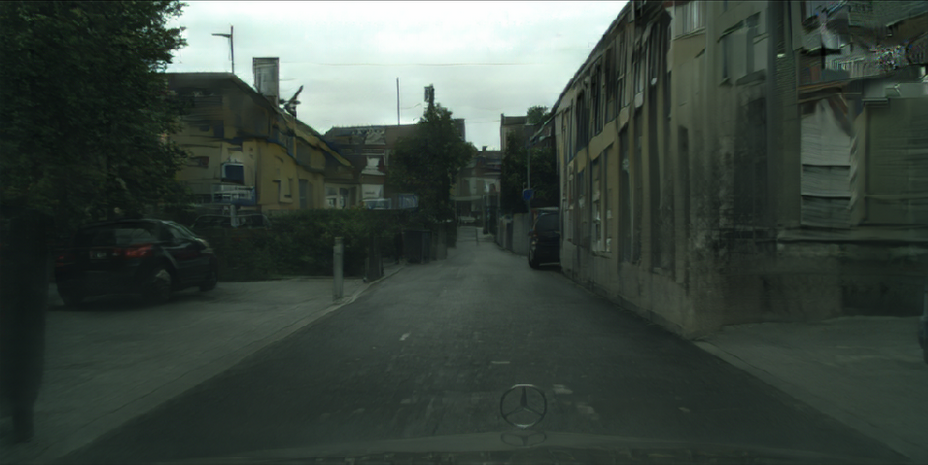
\includegraphics[width=0.9\hsize]{images/golden_colorized_generated.png}
		\label{fig:gan:gen_b}
	}	
	\subfloat{
		\hspace{-4cm}
		\raisebox{11ex}[0pt][0pt]{
			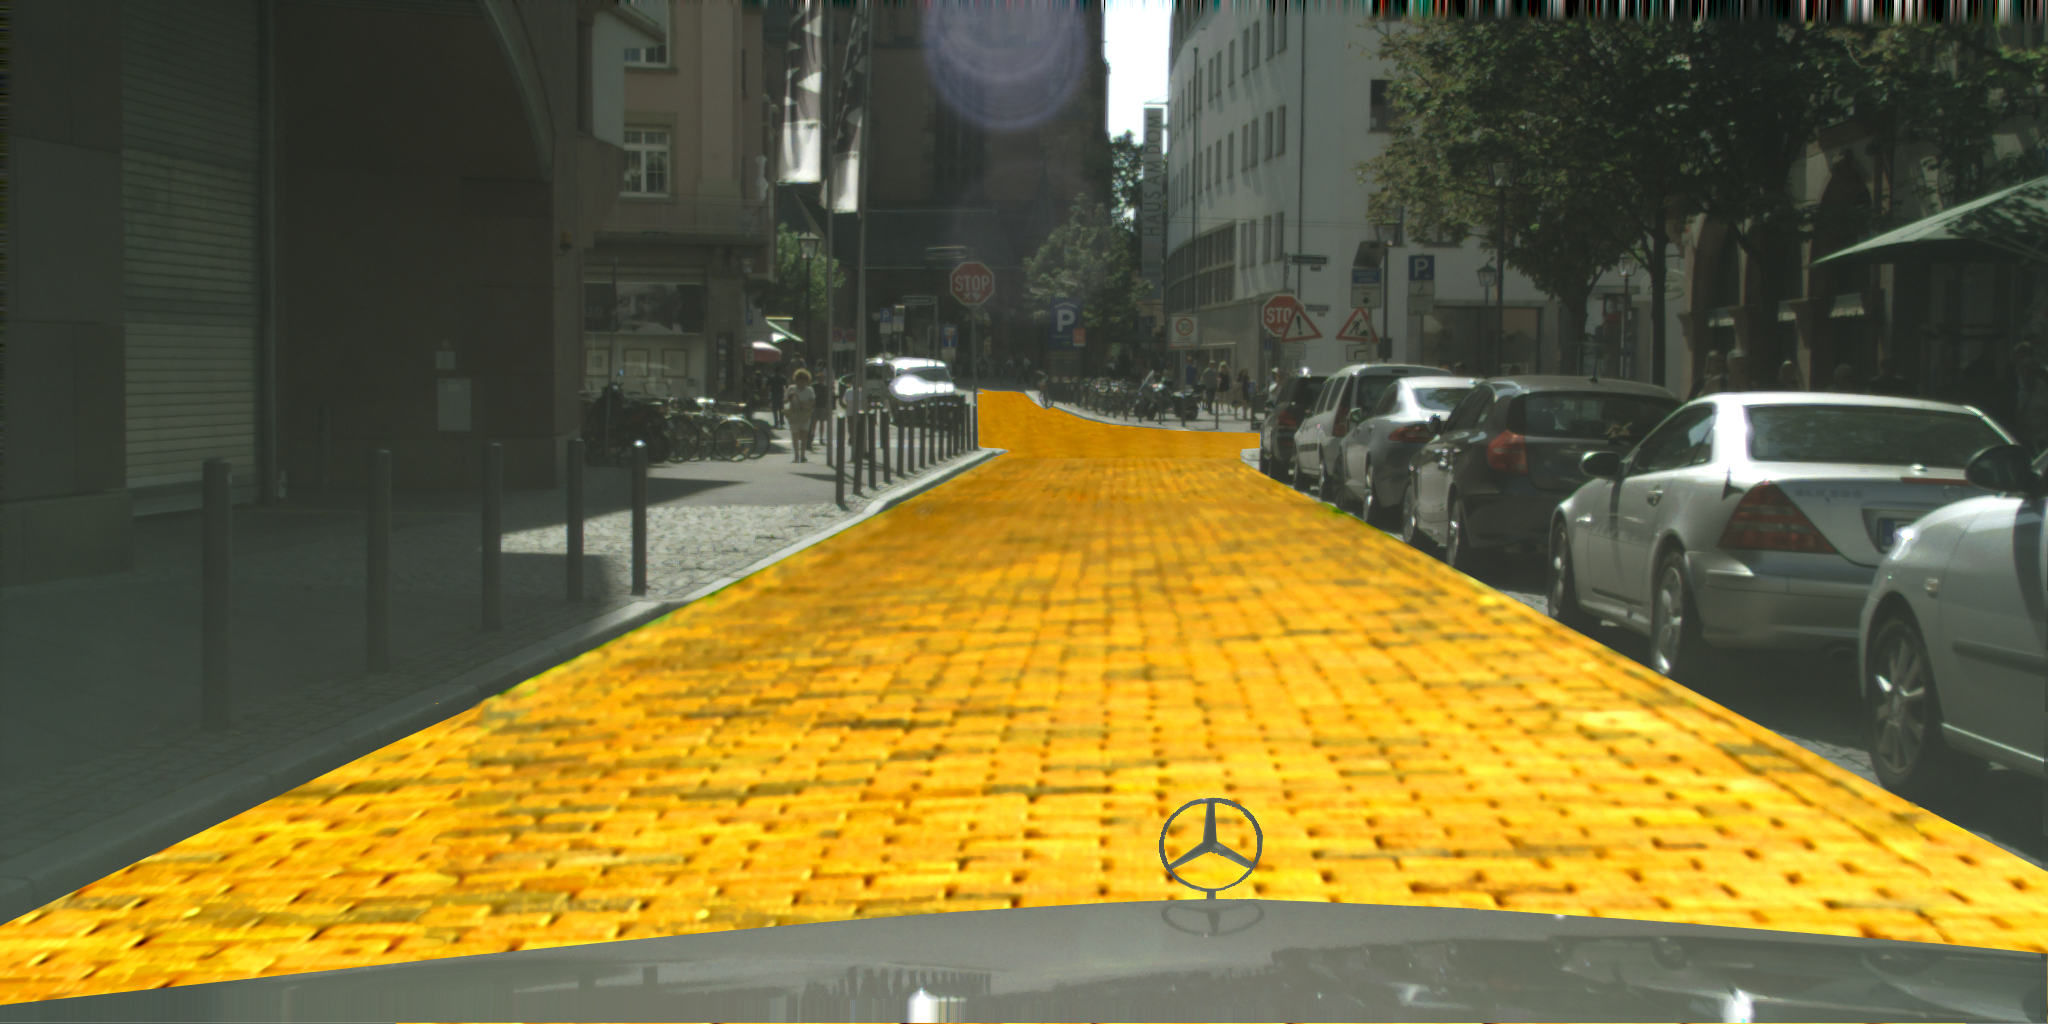
\includegraphics[width=0.5\hsize]{images/manual/result_sat.png}
		}

	}

	\subfloat[Corresponds to blue markers in~\ref{fig:feature_space}. These cobblestones are approximated very well in the generated image.]{
		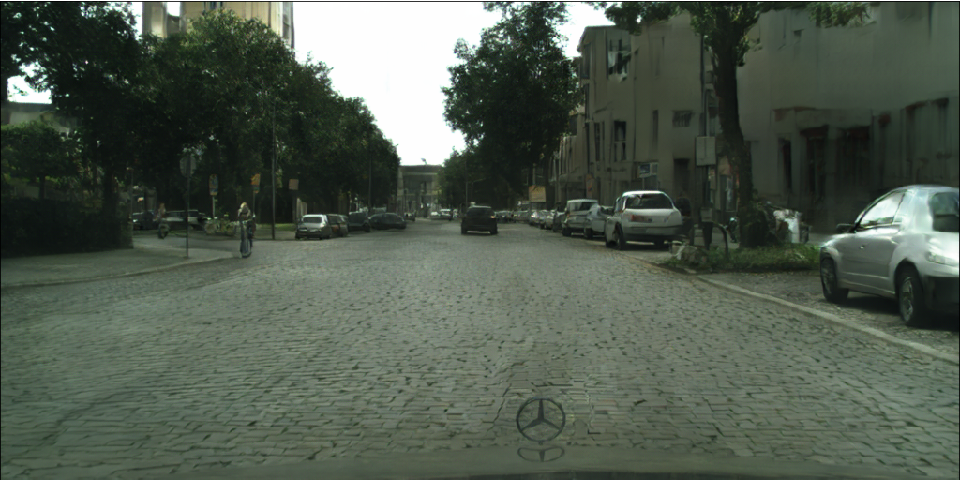
\includegraphics[width=0.9\hsize]{images/color_shift_colorized_generated.png}
		\label{fig:gan:gen_c}
	}	
	\subfloat{
		\hspace{-4cm}
		\raisebox{11ex}[0pt][0pt]{
			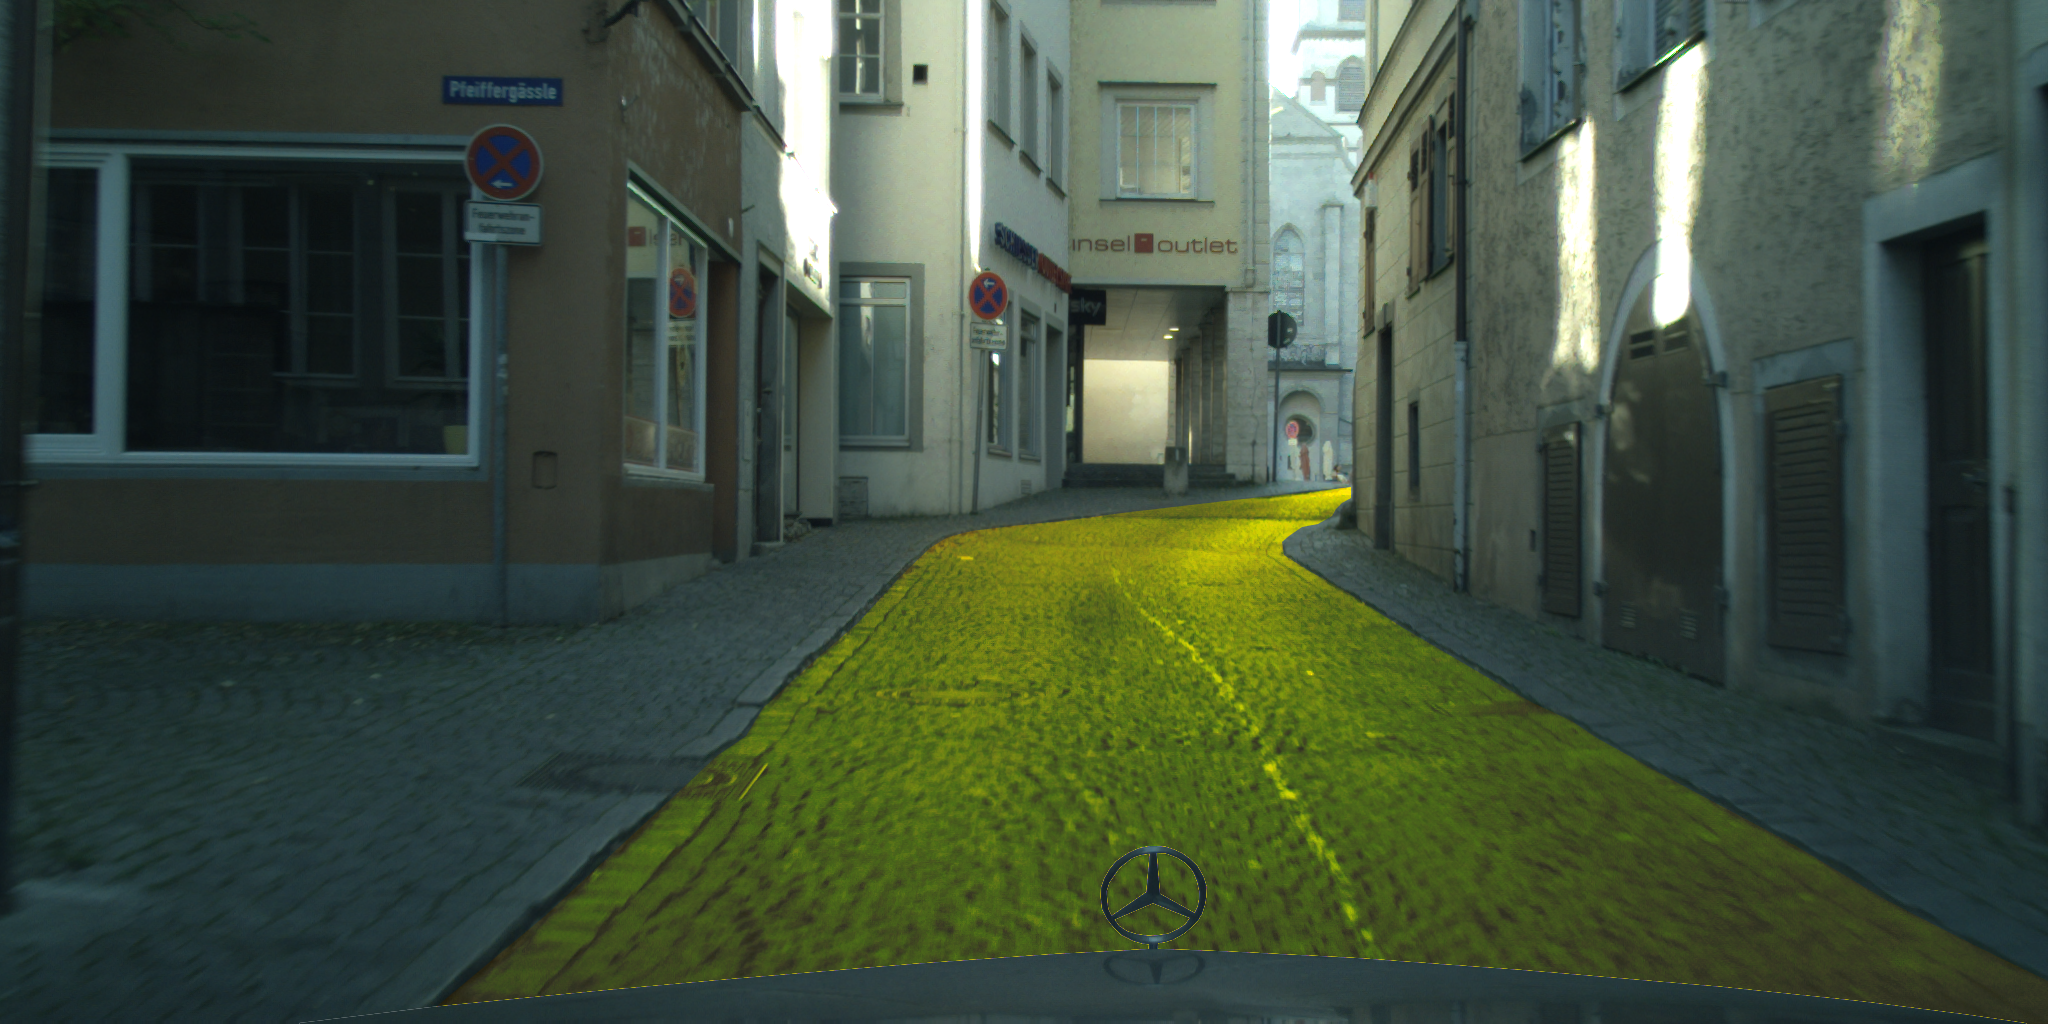
\includegraphics[width=0.5\hsize]{images/manual/colorspace.png}
		}
	}

	\caption{}
	\label{fig:gan}
\end{figure}

Following through with generation using these styles produces results in Figure~\ref{fig:gan}. In two of the cases, regular road textures are produced -- one slate-like road and one cobblestone road. In the third case, no such texture is created. In the feature space plot, we can see that the corresponding purple markers are rather central to the point cloud and are mapped onto relatively standard road patterns.

The last user study involved rating the first and third of the generated images again on realism and similarity to yellow brick roads. Table~\ref{tab:gan} shows that participants consider the generated images extremely realistic, but of course they are not at all like yellow brick roads.



\begin{table}[htb]
\caption{Mean $\pm$ 1 standard deviation survey responses to realism (Q1) and likeness of a `yellow brick road' (Q2) for GAN generated roads, on a scale of 1 to 5. Participants were asked to focus on realism of the road rather than the entire image.}
\vskip 0.15in
\begin{center}
\begin{small}
\begin{sc}
\begin{tabular}{lccr}
\toprule
Figure				 		& Q1				& Q2 			   \\
\midrule
Figure~\ref{fig:gan:gen_a} 	& $3.62 \pm 1.16$	& $1.38 \pm 0.72$  \\
Figure~\ref{fig:gan:gen_c} 	& $4.43 \pm 0.77$	& $1.32 \pm 0.63$  \\
\bottomrule
\end{tabular}
\end{sc}
\end{small}
\end{center}
\vskip -0.1in
\label{tab:gan}
\end{table}

\subsection{Extending the Training Set}

Because GANs are capable of producing such realistic images, a user working on a specific task many times may be willing to provide a few examples of, say, yellow bricks roads, in order to be able to generate similar ones in the future.

Extending training data is an open problem in neural network-driven machine learning~\cite{sarwar2017incremental}. Incremental learning in CNNs typically requires retraining from scratch with the new examples. In our case though, even training 100 epochs of the pix2pixHD GAN takes over 3 days on an NVIDIA Titan X. This is contrary to our goal of making a user-friendly tool.

I attempt to use a novel approach to extending a trained model with new training data. This is inspired by recent work on learning rate schedules~\cite{loshchilov2016sgdr}.

I begin with the trained model from before at epoch 100, and augment  the 2974 training examples with another 6 images -- the manually edited yellow brick roads shown previously along with their grayscale, desaturated road equivalents. I then set the learning rate much higher than the default (which is 0.0002), and modified the training script to decay the learning rate according to a cosine function over 10 or 20 iterations. The idea is to force the model to leave its current local minimum, then quickly settle into a new one that may not be the optimal but good enough.


\begin{figure}
	\subfloat[Cosine Learning Rate Decay, 10 epochs.]{
		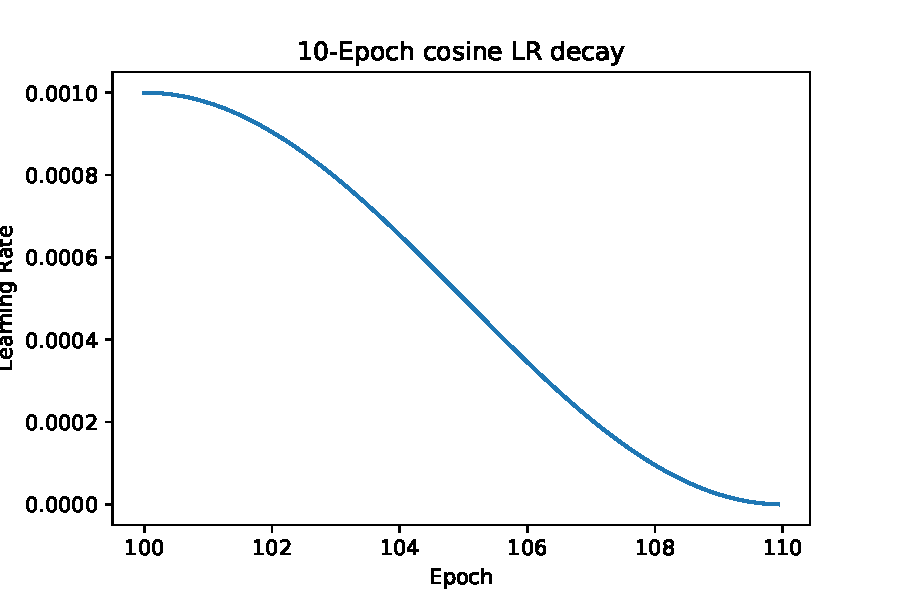
\includegraphics[width=0.5\hsize]{images/10_epoch_cos_decay.pdf}
	}
	\subfloat[Yellow brick road texture to apply (same as in training set for simplicity).]{
		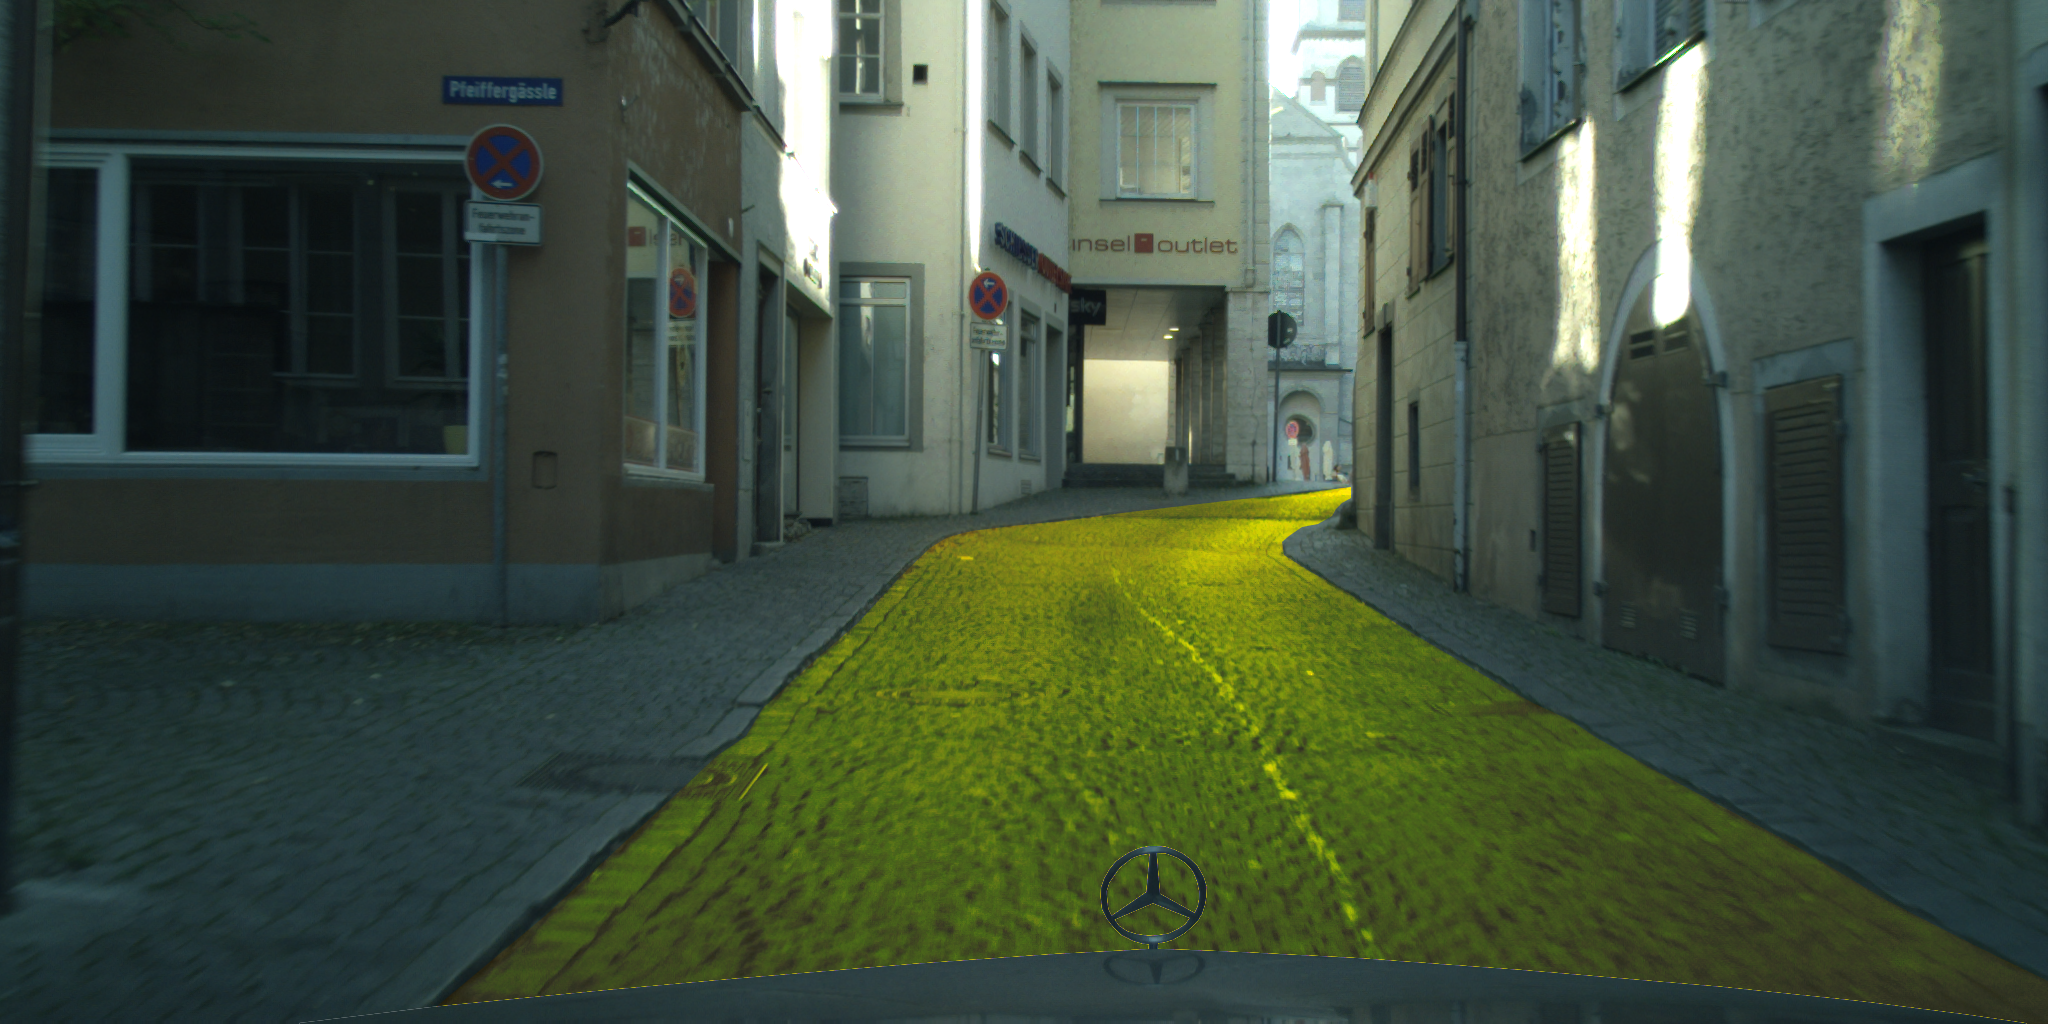
\includegraphics[width=0.5\hsize]{images/manual/colorspace.png}
	}
	
	\subfloat[Generated Image. The overall image is blurrier, and no yellow is produced, but we have certainly left the local minimum found before.]{
		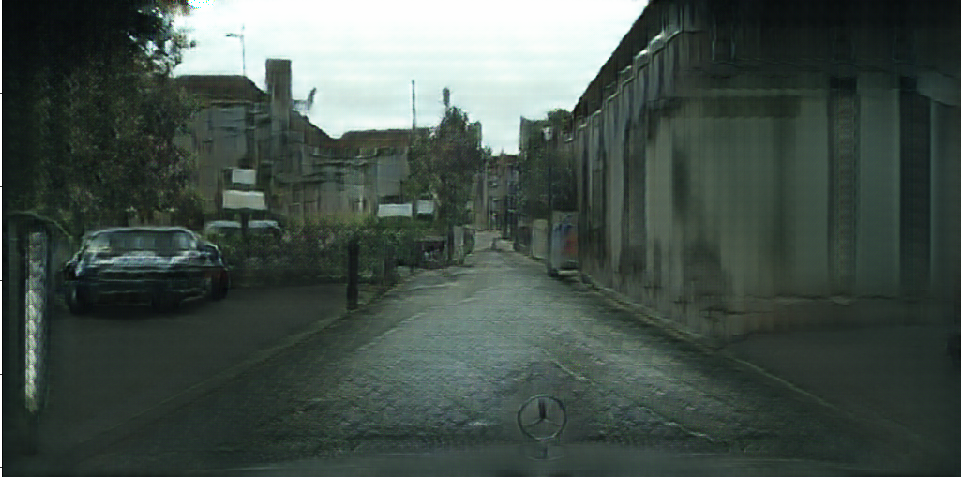
\includegraphics[width=\hsize]{images/cos_10_epoch_color_shift.png}
	}
	\caption{}
	\label{fig:gan:cos_10}
\end{figure}

\begin{figure}

	\subfloat[Cosine Learning Rate Decay, 20 epochs.]{
		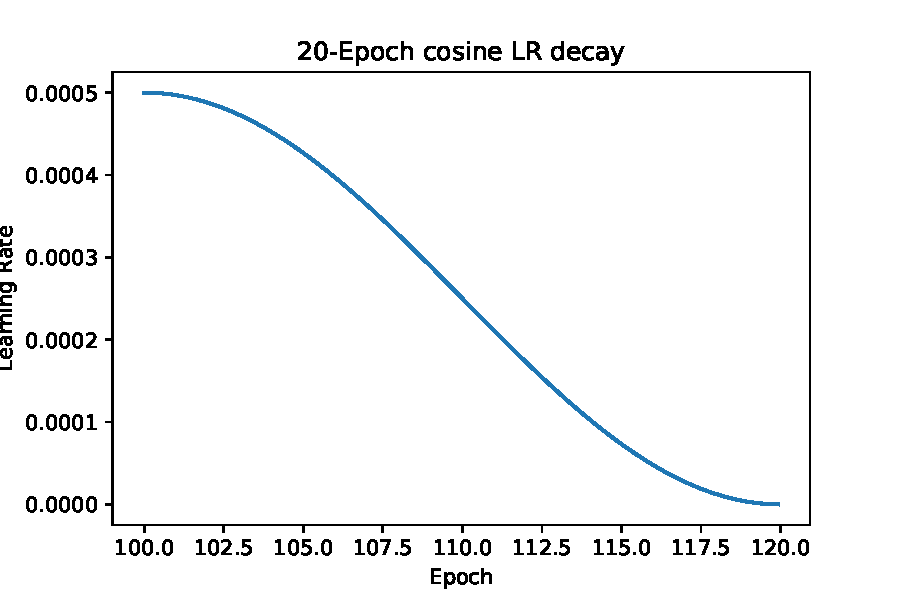
\includegraphics[width=0.5\hsize]{images/20_epoch_cos_decay.pdf}
	}
	\subfloat[Yellow brick road texture to apply (same as in training set for simplicity).]{
		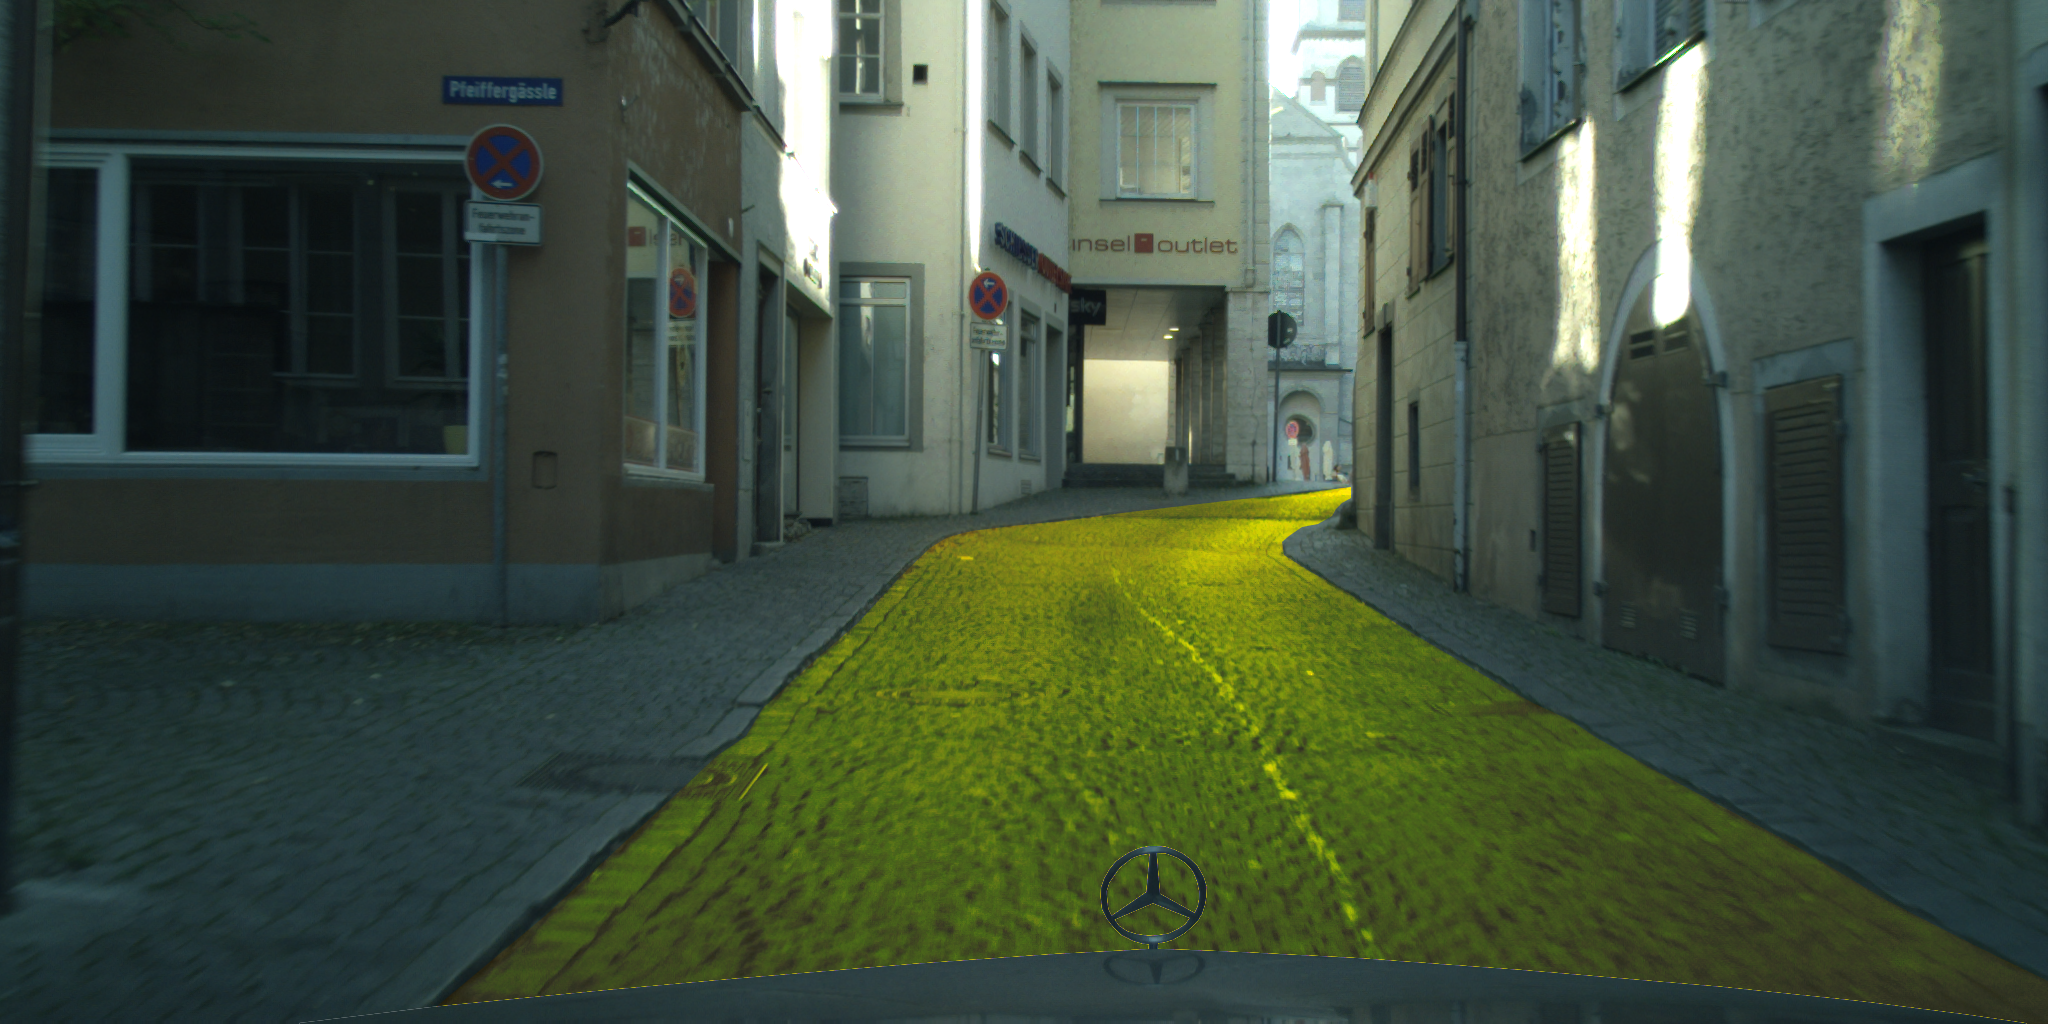
\includegraphics[width=0.5\hsize]{images/manual/colorspace.png}
	}
	
	\subfloat[Generated Image. Most of the image definition has been lost, but amazingly some of the road has acquired yellow hues.]{
		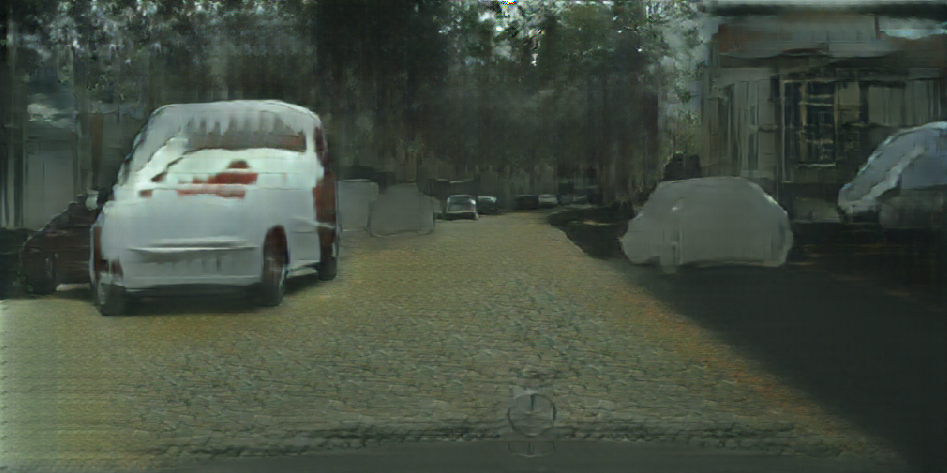
\includegraphics[width=\hsize]{images/cos_20_epoch_color_shift.png}
	}
	\caption{}
	\label{fig:gan:cos_20}

\end{figure}

Neither attempt at using a single, rapid high-to-low cosine decay was particularly successful. A single 10 epoch cycle failed to produce any results besides a snowy-looking road texture in Figure~\ref{fig:gan:cos_10}. Much more interesting is a 20-epoch decay starting with a less aggressive learning rate of 0.0005 (versus 0.001), where yellow tones are visible in the road in Figure~\ref{fig:gan:cos_20}. Unfortunately, definition in all parts of the image has been lost at this point.

Given more GPU time, further investigation would have been performed repeating these attempts, and using multiple, shorter cosine decay cycles to jump between local minima.

Lastly, a full retrain of 100 epochs was completed with the extended dataset. Disappointingly, no yellow was able to be generated from the resulting network. This suggests that 3 color and 3 desaturated examples (on top of 2974 standard examples) of yellow brick roads are not sufficient to expand the GAN's generative capabilities, and that the 20-epoch cosine decay above found a particular local minimum. An interesting research question following from this is approximately how many examples are required to modify a network's generative or predictive capability substantially -- in this case, around 0.1\% is not sufficient to enact even a minor change.


\section{Conclusion}


{\small
\bibliographystyle{ieee}
\bibliography{references}
}

\end{document}
